% This file was converted to LaTeX by Writer2LaTeX ver. 1.4
% see http://writer2latex.sourceforge.net for more info
\documentclass[12pt]{article}
\usepackage[utf8]{inputenc}
\usepackage[T1]{fontenc}
\usepackage[english]{babel}
\usepackage{amsmath}
\usepackage{amssymb,amsfonts,textcomp}
\usepackage{array}
\usepackage{hhline}
\usepackage{hyperref}
\hypersetup{colorlinks=true, linkcolor=blue, citecolor=blue, filecolor=blue, urlcolor=blue}
\usepackage{graphicx}
% footnotes configuration
\makeatletter
\renewcommand\thefootnote{\arabic{footnote}}
\makeatother
\newcommand\textsubscript[1]{\ensuremath{{}_{\text{#1}}}}
\raggedbottom
% Paragraph styles
\renewcommand\familydefault{\rmdefault}
\newenvironment{styleStandard}{\renewcommand\baselinestretch{1.0}\setlength\leftskip{0cm}\setlength\rightskip{0cm plus 1fil}\setlength\parindent{0cm}\setlength\parfillskip{0pt plus 1fil}\setlength\parskip{0in plus 1pt}\writerlistparindent\writerlistleftskip\leavevmode\normalfont\normalsize\writerlistlabel\ignorespaces}{\unskip\vspace{0.111in plus 0.0111in}\par}
\newenvironment{stylelsSectioni}{\renewcommand\baselinestretch{1.0}\setlength\leftskip{0.2957in}\setlength\rightskip{0in plus 1fil}\setlength\parindent{0in}\setlength\parfillskip{0pt plus 1fil}\setlength\parskip{0.1665in plus 0.016649999in}\writerlistparindent\writerlistleftskip\leavevmode\normalfont\normalsize\fontsize{18pt}{21.6pt}\selectfont\bfseries\writerlistlabel\ignorespaces}{\unskip\vspace{0.0835in plus 0.00835in}\par}
\newenvironment{styleinnerExample}{\setlength\leftskip{0.5in}\setlength\rightskip{0in plus 1fil}\setlength\parindent{-0.5in}\setlength\parfillskip{0pt plus 1fil}\setlength\parskip{0cm plus 1pt}\writerlistparindent\writerlistleftskip\leavevmode\normalfont\normalsize\fontsize{10pt}{12.0pt}\selectfont\upshape\writerlistlabel\ignorespaces}{\unskip\vspace{0cm plus 1pt}\par}
\newenvironment{stylelsSectionii}{\renewcommand\baselinestretch{1.0}\setlength\leftskip{0in}\setlength\rightskip{0in plus 1fil}\setlength\parindent{-0.0138in}\setlength\parfillskip{0pt plus 1fil}\setlength\parskip{0.222in plus 0.0222in}\writerlistparindent\writerlistleftskip\leavevmode\normalfont\normalsize\fontsize{16pt}{19.2pt}\selectfont\bfseries\writerlistlabel\ignorespaces}{\unskip\vspace{0.0835in plus 0.00835in}\par}
\newenvironment{styleNormalWeb}{\renewcommand\baselinestretch{1.0}\setlength\leftskip{0cm}\setlength\rightskip{0cm plus 1fil}\setlength\parindent{0cm}\setlength\parfillskip{0pt plus 1fil}\setlength\parskip{0in plus 1pt}\writerlistparindent\writerlistleftskip\leavevmode\normalfont\normalsize\writerlistlabel\ignorespaces}{\unskip\vspace{0.111in plus 0.0111in}\par}
% List styles
\newcommand\writerlistleftskip{}
\newcommand\writerlistparindent{}
\newcommand\writerlistlabel{}
\newcommand\writerlistremovelabel{\aftergroup\let\aftergroup\writerlistparindent\aftergroup\relax\aftergroup\let\aftergroup\writerlistlabel\aftergroup\relax}
\newcounter{listWWNumxxivleveli}
\newcounter{listWWNumxxivlevelii}[listWWNumxxivleveli]
\newcounter{listWWNumxxivleveliii}[listWWNumxxivlevelii]
\newcounter{listWWNumxxivleveliv}[listWWNumxxivleveliii]
\renewcommand\thelistWWNumxxivleveli{\arabic{listWWNumxxivleveli}}
\renewcommand\thelistWWNumxxivlevelii{\arabic{listWWNumxxivleveli}.\arabic{listWWNumxxivlevelii}}
\renewcommand\thelistWWNumxxivleveliii{\arabic{listWWNumxxivleveli}.\arabic{listWWNumxxivlevelii}.\arabic{listWWNumxxivleveliii}}
\renewcommand\thelistWWNumxxivleveliv{\arabic{listWWNumxxivleveli}.\arabic{listWWNumxxivlevelii}.\arabic{listWWNumxxivleveliii}.\arabic{listWWNumxxivleveliv}}
\newcommand\labellistWWNumxxivleveli{\thelistWWNumxxivleveli.}
\newcommand\labellistWWNumxxivlevelii{\thelistWWNumxxivlevelii.}
\newcommand\labellistWWNumxxivleveliii{\thelistWWNumxxivleveliii.}
\newcommand\labellistWWNumxxivleveliv{\thelistWWNumxxivleveliv.}
\newenvironment{listWWNumxxivleveli}{\def\writerlistleftskip{\setlength\leftskip{0.5in}}\def\writerlistparindent{}\def\writerlistlabel{}\def\item{\def\writerlistparindent{\setlength\parindent{-0.25in}}\def\writerlistlabel{\stepcounter{listWWNumxxivleveli}\makebox[0cm][l]{\labellistWWNumxxivleveli}\hspace{-0.635cm}\writerlistremovelabel}}}{}
\newenvironment{listWWNumxxivlevelii}{\def\writerlistleftskip{\setlength\leftskip{1in}}\def\writerlistparindent{}\def\writerlistlabel{}\def\item{\def\writerlistparindent{\setlength\parindent{-0.25in}}\def\writerlistlabel{\stepcounter{listWWNumxxivlevelii}\makebox[0cm][l]{\labellistWWNumxxivlevelii}\hspace{-1.905cm}\writerlistremovelabel}}}{}
\newenvironment{listWWNumxxivleveliii}{\def\writerlistleftskip{\setlength\leftskip{1.5in}}\def\writerlistparindent{}\def\writerlistlabel{}\def\item{\def\writerlistparindent{\setlength\parindent{-0.1252in}}\def\writerlistlabel{\stepcounter{listWWNumxxivleveliii}\makebox[0cm][r]{\labellistWWNumxxivleveliii}\hspace{-3.4919918cm}\writerlistremovelabel}}}{}
\newenvironment{listWWNumxxivleveliv}{\def\writerlistleftskip{\setlength\leftskip{2in}}\def\writerlistparindent{}\def\writerlistlabel{}\def\item{\def\writerlistparindent{\setlength\parindent{-0.25in}}\def\writerlistlabel{\stepcounter{listWWNumxxivleveliv}\makebox[0cm][l]{\labellistWWNumxxivleveliv}\hspace{-4.4449997cm}\writerlistremovelabel}}}{}
\title{}
\author{Anna}
\date{2019-07-23}
\begin{document}
\title{\ The puzzle of Russian ditransitives}
\maketitle

\begin{styleStandard}
\textbf{Svitlana Antonyuk}
\end{styleStandard}

\begin{styleStandard}
\textbf{\ University of Connecticut}\footnote{* I gratefully acknowledge helpful feedback and suggestions for improvement I received from John F. Bailyn, Richard K. Larson, Viviane Deprez, Gillian Ramchand, Alec Marantz and Peter Hallman that led to significant improvement of this paper, as well as helpful criticisms and questions of two anonymous reviewers. This research was supported by~Austrian Science Fund (FWF), Grant~number: P27384-G23 awarded to Dr. Peter Hallman.}
\end{styleStandard}

\begin{styleStandard}
\textbf{\textit{Abstract}}\textit{. In this paper I use the Scope Freezing Generalization (SFG), formulated on the basis of Russian quantifier scope freezing data in Antonyuk (2015) to gain insights into the structure of Russian ditransitives. The paper discusses the finding that Russian ditransitive predicates are not a homogeneous group, but instead subdivide into three distinct Groups, each with its distinct set of properties, with further syntactic evidence supporting the conclusion that these Groups have distinct underlying structures. One of the main findings, suggested by the (revised) SFG and supported by syntactic unaccusativity tests is that a group of Russian “direct objects” are not in fact what they seem, but are instead low Oblique arguments receiving Accusative case from a silent P head.}
\end{styleStandard}

\begin{styleStandard}
\textbf{Keywords:} \textit{ditransitives, scope freezing, Russian, unaccusativity, objecthood, Oblique Accusatives.}
\end{styleStandard}


\setcounter{listWWNumxxivleveli}{0}
\begin{listWWNumxxivleveli}
\item 
\begin{stylelsSectioni}
Introduction
\end{stylelsSectioni}
\end{listWWNumxxivleveli}
\begin{styleStandard}
The argument structure of ditransitive predicates has been of interests to linguists for quite a long time, with the question of the exact nature of syntactic encoding of ditransitives remaining both a matter of debate and a source of important insights for grammatical theory. Thus, even in English, which has been studied extensively in the generative tradition for over half a century the question of argument structure is far from settled, with novel research ranging in analyses from a derivational Larsonian view (Larson 1988; 2014) to separate projection view (an applicative analysis of Marantz 1993; decompositional analyses of Pesetsky 1995; Harley 1995; 2002 i.a.) to a derivational reverse-Larsonian view on which the Double Object Construction (DOC) serves as the derivational base for the Prepositional Dative Construction (Hallman 2015). It is not surprising then that in languages that have not been studied as extensively within the generative framework, Russian being one of them, there is little to no agreement on the issue, with a variety of views, schematized in (1) below:
\end{styleStandard}

\begin{styleStandard}
(1) Analyses of Russian ditransitives:
\end{styleStandard}

\begin{styleStandard}
a. \textbf{Dative Goal object originates in Spec, VP position}, assigned Dative case as sister to V’ (see Harbert \& Toribio 1991; Greenberg \& Franks 1991; Franks 1995 Richardson 2007)
\end{styleStandard}

\begin{styleStandard}
b. \textbf{Accusative Theme object is generated in Spec, VP position}, with the Dative originating in the complement position (Bailyn 1995, 2010, 2012; Titov 2017)\newline
\newline
c. \textbf{Dative Goal object is assigned case by an Applicative head} (Dyakonova 2005, 2007, following Pylkkänen 2002)
\end{styleStandard}

\begin{styleStandard}
d. \textbf{Non-derivational Dative-higher-than-Theme account} of ditransitves on which datives (locational vs. non-locational) have two distinct underlying structures (Boneh \& Nash 2017)
\end{styleStandard}

\begin{styleStandard}
The research summarized here, developed in detail in Antonyuk (2015) offers a way to understand the reason behind such multitude of views on Russian ditransitives by presenting a novel perspective, different from all of the above in that it discards the underlying assumption of the uniformity of Russian ditransitives and argues instead that Russian ditransitive predicates subdivide into three distinct Groups, each with its own clearly defined set of properties and corresponding differences in syntactic structure. The initial evidence for this proposal comes from quantifier scope ambiguity and scope freezing distribution patterns in ditransitives, supported further by syntactic tests that confirm the underlying structural differences between the three Groups.
\end{styleStandard}

\begin{styleStandard}
The insight about the non-homogeneous nature of Russian ditransitives comes primarily from the scope ambiguity and scope freezing distribution patterns and it should be stressed that the notion of ditransitivity that emerges from this investigation is broader than what is generally assumed. In research on English, for instance, the notion of ditransitivity has been reserved mostly for verbs that undergo Dative shift (the prepositional Dative and the Double Object Construction), as well as the \textit{Spray-Load} alternation. The Double Object Construction and the \textit{with}{}-variant of the \textit{Spray-Load} alternation are also the constructions that exhibit the scope freezing phenomenon in English (differing in this respect from the scopally ambiguous Prepositional Dative Construction and the other alternant of the \textit{Spray-Load} alternation), with scope ambiguity-scope freezing contrast being treated as one of the properties that characterize ditransitives in English (see, for instance, Bruening 2001, 2010). Current research takes the view that the scope ambiguity - scope freezing contrast is one of the most important properties of ditransitive verbs and moreover, that the scope ambiguity-scope freezing distribution patterns can be used to gain insights into the argument structure of ditransitives. The operative notion of ditransitivity, therefore, has been derived entirely on the basis of which predicates exhibit the scope ambiguity - scope freezing distribution patterns, and that appears to include any predicate which Theta-marks two internal arguments. Thus, the relevant notion of ditransitivity is one that includes both the “canonical” ditransitives which take an Accusative-marked Theme and a Dative-marked Goal internal arguments as well as verbs which include an Accusative-marked Theme and a PP argument or an Instrumental-marked DP or even those where the verbs subcategorizes for two internal arguments which are both realized as Prepositional Phrases. 
\end{styleStandard}

\begin{styleStandard}
Turning to data now, despite arguably being identical to English in terms of quantifier scope possibilities and Quantifier Raising properties as far as transitive sentences are concerned (see Antonyuk-Yudina 2006; Antonyuk 2015; 2019) there are both significant similarities \textit{and} differences once we look at ditransitive sentences. While the important similarity to English is that Russian ditransitives show the same scope freezing effect as do English DOCs and the \textit{with}{}-variant of the \textit{Spray-Load} construction, the novel Russian data, briefly exemplified in (2)-(7) below, suggest that the range of constructions in which quantifier scope is surface scope frozen in the language is much broader than it is in English. In all of the examples below the sentences in (a) are ambiguous, whereas the sentences in (b) are surface scope frozen. 
\end{styleStandard}

\begin{styleStandard}
(2)\textbf{ }Russian Equivalent of the PP Dative and the Double-Object Construction: 
\end{styleStandard}

\begin{styleinnerExample}
a.\ \ \textit{Učitel’. \ \ \ \ \ \ \ \ podaril \ \ \ \ \ kakuju-to \ \ knigu\ \  \ \ \ \ \ \ \ \ \ \ každomu}
\end{styleinnerExample}

\begin{styleinnerExample}
\ \ Teacher\textsc{nom} presented [some \ \ book]\textsc{acc.fem \ }[every \ 
\end{styleinnerExample}

\begin{styleinnerExample}
\textit{\ \ studentu}
\end{styleinnerExample}

\begin{styleinnerExample}
\ \ student]\textsc{dat.msc}\textbf{\textsubscript{ }}
\end{styleinnerExample}

\begin{styleinnerExample}
\ \ “The teacher presented some book to every student” ${\exists}{\forall}$/${\forall}{\exists}$
\end{styleinnerExample}

\begin{styleinnerExample}
b.\ \ \textit{Učitel’ \ \ \ \ \ \ \ \ \ podaril \ \ \ \ \ kakomu-to student \ \ \ \ každuju}
\end{styleinnerExample}

\begin{styleinnerExample}
\ \ Teacher\textsc{nom} presented [some \ \ \ \ \ \ \ \ student]\textsc{dat.msc \ \ }[every \newline
knigu.\newline
book]\textsc{acc.fem}\newline
“The teacher presented some student with every book” ${\exists}{\forall}$/*${\forall}{\exists}$
\end{styleinnerExample}

\begin{styleStandard}
(3)\textbf{ }Prepositional Ditransitive Construction:
\end{styleStandard}

\begin{styleinnerExample}
a.\ \ \textit{Maša \ \ potrebovala \ [kakie-to dokumenty] \ \ \ \ \ \ \ (s \ \ \ \ \ \ každogo \ }
\end{styleinnerExample}

\begin{styleinnerExample}
Masha demanded \ \ \ \ [some documents] \textsc{acc }[\textsubscript{PP} from every \newline
posetitelja)\newline
visitor]\textsc{gen}
\end{styleinnerExample}

\begin{styleinnerExample}
\ \ “Masha demanded some documents from every visitor” \ ${\exists}{\forall}$/${\forall}{\exists}$
\end{styleinnerExample}

\begin{styleinnerExample}
b.\ \ \textit{Maša \ \ potrebovala \ \ (s kakogo-to posetitelija) [každyj document]}
\end{styleinnerExample}

\begin{styleinnerExample}
\ \ Masha demanded [\textsubscript{PP} from some \ \ visitor] \textsc{gen} [every \ \ document] \textsc{acc}
\end{styleinnerExample}

\begin{styleinnerExample}
\ \ “Masha demanded every document from some visitor” ${\exists}{\forall}$/*${\forall}{\exists}$
\end{styleinnerExample}

\begin{styleStandard}
(4)\textbf{ }The \textit{Spray-Load} Alternation:
\end{styleStandard}

\begin{styleinnerExample}
a.\ \ \textit{Vanja zagruzil [kakoj-to \ \ \ vid \ \ sena] \ \ \ \ \ \ [na \ každyj gruzovik]}
\end{styleinnerExample}

\begin{styleinnerExample}
\ \ Vania loaded \ \ [some \ \ type hay] \textsc{gen} [on [every \ truck] \textsc{acc}]
\end{styleinnerExample}

\begin{styleinnerExample}
\ \ “Vania loaded some type of hay on every truck” ${\exists}{\forall}$/${\forall}{\exists}$
\end{styleinnerExample}

\begin{styleinnerExample}
b.\ \ \textit{Vanja zagruzil [kakoj-to gruzovik] \ \ \ [každym vidom \ \  \ \ \ \ \ \ sena]}
\end{styleinnerExample}

\begin{styleinnerExample}
\ \ Vania loaded \ [some \ \ \ \ \ \ truck] \textsc{acc} [[every \ \ \ type]\textsc{ instr} \ hay-\textsc{gen}]
\end{styleinnerExample}

\begin{styleinnerExample}
\ \ “Vania loaded some truck with every type of hay” ${\exists}{\forall}$/*${\forall}{\exists}$
\end{styleinnerExample}

\begin{styleStandard}
(5)\textbf{ }The \textit{Clear}{}-Type Alternation: 
\end{styleStandard}

\begin{styleinnerExample}
a.\ \ \textit{Vanja ubral \ \ \ [neskol’ko \ tarelok]\ \  \ \ \ [s \ \ \ \ \ \ \ každogo stola]}
\end{styleinnerExample}

\begin{styleinnerExample}
\ \ Vania cleared [several \ \ \ \ \ dishes] \textsc{acc} [from [every \ \ \ \ \ table] \textsc{acc]}
\end{styleinnerExample}

\begin{styleinnerExample}
\ \ “Vania cleared several dishes from every table” ${\exists}{\forall}$/${\forall}{\exists}$
\end{styleinnerExample}

\begin{styleinnerExample}
b.\ \ \textit{Vanja ubral \ \ [neskol’ko stolov]\ \  \ \ \ [ot \ \  každoj tarelki]}
\end{styleinnerExample}

\begin{styleinnerExample}
\ \ Vania cleared [several. \ \ \ \ tables] \textsc{acc} \ [from\ \ [every \ dish] \textsc{gen}]\newline
“Vania cleared several tables of every dish” ${\exists}{\forall}$/*${\forall}{\exists}$
\end{styleinnerExample}

\begin{styleStandard}
(6)\textbf{ }Simple Ditransitives:
\end{styleStandard}

\begin{styleinnerExample}
a.\ \ \textit{Maša \ \ zarazila [kakoj-to bolezn’ju]\ \ [každogo pacienta]}
\end{styleinnerExample}

\begin{styleinnerExample}
\ \ Masha infected [some \ \ \ \ \ illness] \textsc{instr} \ \ [every \ \ \ \ patient] \textsc{acc}
\end{styleinnerExample}

\begin{styleinnerExample}
\ \ “Masha infected with some illness every patient” \textit{${\exists}{\forall}$/${\forall}{\exists}$}
\end{styleinnerExample}

\begin{styleinnerExample}
b.\ \ \textit{Maša \ \ zarazila [kakogo-to pacienta] \ \ [každoj bolezn’ju]}
\end{styleinnerExample}

\begin{styleinnerExample}
\ \ Masha infected [some \ \ \ \ \ \ \ \ patient] \textsc{acc} \ \ [every \ illness]\textsc{instr}
\end{styleinnerExample}

\begin{styleinnerExample}
\ \ “Masha got infected with every illness by some patient” ${\exists}{\forall}$/*${\forall}{\exists}$
\end{styleinnerExample}

\begin{styleStandard}
(7)\textbf{ }“Reflexive Monotransitives” derived from simple ditransitives:
\end{styleStandard}

\begin{styleinnerExample}
a.\ \ \textit{Maša \ \ zarazilas’\ \  \ \ \ \ \ \ [kakoj-to bolezn’ju] [ot \ \ \ \ \ každogo pacienta]}
\end{styleinnerExample}

\begin{styleinnerExample}
\ \ Masha infected-\textsc{refl \ }[some illness] \textsc{instr} [from [every \ \ \ \ patient]\textsc{gen }“Masha got infected with some illness by every patient” ${\exists}{\forall}$/${\forall}{\exists}$\newline

\end{styleinnerExample}

\begin{styleinnerExample}
b.\ \ \textit{Maša \ \ zarazilas’ \ \  \ \ \ \ \ \ [ot \ \ \ \ \ kakogo-to pacienta] \ \ \ \ \ [každoj }
\end{styleinnerExample}

\begin{styleinnerExample}
\ \ Masha infected-\textsc{refl \ \ }[from [some \ \  \ \ \ \ \ patient]\textsc{gen ]} [every 
\end{styleinnerExample}

\begin{styleinnerExample}
\ \ bolezn’ju]
\end{styleinnerExample}

\begin{styleinnerExample}
\ \ illness]\textsc{instr}
\end{styleinnerExample}

\begin{styleinnerExample}
\ \ “Masha got infected with every illness by some patient” ${\exists}{\forall}$/*${\forall}{\exists}$
\end{styleinnerExample}

\begin{styleStandard}
What is striking about the above examples is that despite all the differences between these sentences, such as changes in the obligatory morphological marking between the two alternating orders in the \textit{Spray-Load} or \textit{Clear}{}-type alternations or the fact that in some cases one of the internal arguments is realized as a Prepositional Phrase (PP) or, perhaps most strikingly, the “detransitivization” in (7) with scope freezing nevertheless preserved, all the differences notwithstanding, the one constant element in the above pairs is the permuted order of the verb’s internal arguments. The Scope Freezing Generalization in (8) captures this fact:\footnote{ The SGF in (8) reflects the important assumption that scope ambiguity is the norm and scope freezing is the “marked”, special case in need of an explanation. }\textsuperscript{,}\footnote{ In this paper I argue, contra Antonyuk (2015), that surface scope freezing observed with ditransitives and captured by SFG in (8) is a categorically distinct phenomenon from the surface scope \textit{bias }found with cases of scrambling of a QP across a higher QP, as the judgments of surface scope freezing found with Groups 1 and 2 are not similarly affected by Information Structure-relevant phenomena such as prosodically realized Contrastive Focus (Antonyuk and Larson 2016) or by Specificity-related Object Shift, as demonstrated for Ukrainian in Antonyuk and Mykhaylyk (under review).}
\end{styleStandard}

\begin{styleStandard}
(8)\textbf{ }Scope Freezing Generalization (SFG), revised (cf. Antonyuk 2015): 
\end{styleStandard}

\begin{styleStandard}
\textit{Scope freezing results when one QP raises over another to a c-commanding position within the VP as a result of a single instance of movement.}
\end{styleStandard}

\begin{styleStandard}
\newline
In section 2 I use the scope data and the SF Generalization as a diagnostic, which suggests a non-homogeneous view of Russian ditransitives according to which they subdivide into 3 distinct Groups. In section 3 I discuss syntactic evidence supporting the claim that these groups are distinct. Section 4 describes which structural possibilities are open for each group of Russian ditransitives, based on observed data patterns. Section 5 concludes the paper. 
\end{styleStandard}

\begin{listWWNumxxivleveli}
\item 
\begin{stylelsSectioni}
The basic empirical generalization: 3 classes of Russian ditransitives 
\end{stylelsSectioni}
\end{listWWNumxxivleveli}
\begin{styleStandard}
Most of the Russian ditransitive~constructions can be said to share the property of taking an Accusative (ACC) and a Non-Structural (Inherent) case-marked argument (marked here throughout as OBL for Oblique) that can occur in either order in surface form. The two orders of internal arguments are always truth-conditionally identical, with subtle information-structural distinctions between them. Here the Groups are distinguished according to the effect that word order permutations have on their scope interpretation possibilities. Thus, based on their scope behavior alone, we can distinguish between three distinct classes of ditransitives in Russian, schematized below:
\end{styleStandard}

\begin{styleStandard}
(9)\ \ \textbf{Group 1}\ \ \ \ \ \ (10)\ \ \textbf{Group 2}\newline
ACC {\textgreater} OBL ~(ambiguous) \ \ \ \ OBL {\textgreater} ACC(ambiguous)\newline
OBL {\textgreater} ACC ~(frozen) \ \ \ \ ACC {\textgreater} OBL ~(frozen)
\end{styleStandard}

\begin{styleStandard}
(11)\ \ \textbf{Group 3}\newline
ACC {\textgreater} OBL ~(ambiguous)\newline
OBL {\textgreater} ACC ~(ambiguous)
\end{styleStandard}

\begin{listWWNumxxivleveli}
\item 
\begin{listWWNumxxivlevelii}
\item 
\begin{stylelsSectionii}
The three groups exemplified
\end{stylelsSectionii}
\end{listWWNumxxivlevelii}
\end{listWWNumxxivleveli}
\begin{styleStandard}
Group 1 is exemplified by Russian verbs such as \textit{podarit’} ('to present’), which most often selects an Accusative Theme and a Dative Recipient argument: \footnote{ Throughout this paper, the phrase in square brackets represents the argument that cannot be dropped/elided. The one in parenthesis may be omitted while still being implicitly understood. }
\end{styleStandard}

\begin{styleinnerExample}
(12)\ \ a.\ \ \textit{Vospitatel’ \ \ \ \ \ podaril \ \ [kakuju-to igrušku]. \ \ \ \ \ \ [každomu} 
\end{styleinnerExample}

\begin{styleinnerExample}
\ \ \ \ Caretaker\textsc{nom} presented \ \ [some \ \  \ \ \ toy]\textsc{acc.fem }[every
\end{styleinnerExample}

\begin{styleinnerExample}
\ \ \ \ \textit{rebjenku]}
\end{styleinnerExample}

\begin{styleinnerExample}
\ \ \ \ child]\textsc{dat.msc}
\end{styleinnerExample}

\begin{styleinnerExample}
\ \ \ \ “The teacher presented some book to every student” ${\exists}{\forall}$/${\forall}{\exists}$
\end{styleinnerExample}

\begin{styleinnerExample}
\ \ b.\ \ \textit{Vospitatel’ \ \ \ \ \ \ podaril \ \ [kakomu-to rebjenku] \ \  [každuju }
\end{styleinnerExample}

\begin{styleinnerExample}
\ \ \ \ Caretaker\textsc{nom} \ presented \ \ [some \ \  \ \ \ \ child]\textsc{dat.msc }[every \ \newline
\textit{igrušku]}
\end{styleinnerExample}

\begin{styleinnerExample}
\ \ \ \ toy]acc.fem
\end{styleinnerExample}

\begin{styleinnerExample}
\ \ \ \ “The caretaker presented some child with every toy” ${\exists}{\forall}$/*${\forall}{\exists}$
\end{styleinnerExample}

\begin{styleStandard}
The alternation in (12a,b) resembles the scope freezing pattern of English alternating ditransitives. As we know from English, the THEME \ {\textgreater} \ GOAL/RECIPIENT order of quantifiers is ambiguous (13a), allowing either quantifier to be read with wide scope. However, the GOAL/RECIPIENT {\textgreater} THEME order is frozen (13b), allowing only the surface scope interpretation (Larson 1990, Bruening 2001).\newline

\end{styleStandard}

\begin{styleinnerExample}
(13) \ \ a.\ \ Alice assigned some exercise to every student.~${\exists}{\forall}$/${\forall}{\exists}$\newline
b.\ \ Alice assigned some student every~exercise.~ ${\exists}{\forall}$/*${\forall}{\exists}$
\end{styleinnerExample}

\begin{styleStandard}
(14) presents a non-exhaustive list of verbs whose behavior with respect to the scope freezing diagnostic places them into Group 1:
\end{styleStandard}

\begin{styleinnerExample}
(14)\textbf{ \ \ }a. \ \ dat’ ACC/DAT \ {}- to give (something to.somebody)
\end{styleinnerExample}

\begin{styleinnerExample}
\ \ b. \ \ poobeščat’ACC/DAT – to promise (something to.somebody)
\end{styleinnerExample}

\begin{styleinnerExample}
\ \ c.\ \ zaveščat’ ACC/DAT – to bequeath (something to.somebody)
\end{styleinnerExample}

\begin{styleinnerExample}
\ \ d.\ \ najti ACC/DAT – to find (something for.someone);
\end{styleinnerExample}

\begin{styleinnerExample}
\ \ e. \ \ prostit’ ACC/DAT – to forgive (something to.someone);
\end{styleinnerExample}

\begin{styleinnerExample}
\ \ f. \ \ napisat’ ACC/DAT or ACC/k DAT – to write (something to.someone or something to someone)
\end{styleinnerExample}

\begin{styleinnerExample}
\ \ g. \ \ sdelat’ ACC/DAT – to do (something to.somebody);
\end{styleinnerExample}

\begin{styleinnerExample}
\ \ h. \ \ predložit’ ACC/DAT – to offer (something to.someone);
\end{styleinnerExample}

\begin{styleinnerExample}
\ \ i. \ \ ostavit’ ACC/DAT \ {}- to leave (something to.somebody);
\end{styleinnerExample}

\begin{styleinnerExample}
\ \ j. \ \ potrebovat ACC/s ACC – to demand (something from someone);
\end{styleinnerExample}

\begin{styleinnerExample}
\ \ k. \ \ zaključit’ pari/s INSTR – to place a bet with someone.
\end{styleinnerExample}

\begin{styleStandard}
The example in (15) presents a Group 2 verb on its two alternating orders. Here, the order on which the Instrumental-marked phrase precedes the Accusative argument is scopally ambiguous, whereas the opposite order of arguments is surface scope frozen. 
\end{styleStandard}

\begin{styleinnerExample}
(15)\textbf{\ \ }a.\ \ \textit{Maša \ \ ugostila (kakim-to pečenjem) \ \ \ \ \ \ [každogo rebenka]}
\end{styleinnerExample}

\begin{styleinnerExample}
\ \ \ \ Masha treated \ [some \ \ \ \ \ \ \ cookie]\textsc{instr ~} [every \ \ \ \ child]\textsc{acc}
\end{styleinnerExample}

\begin{styleinnerExample}
\ \ \ \ “Masha treated every child to some cookie” ${\exists}{\forall}$/${\forall}{\exists}$
\end{styleinnerExample}

\begin{styleinnerExample}
\ \ b.\ \ \textit{Maša \ \ ugostila [kakogo-to rebenka] \ \ \ (každym pečenjem)}
\end{styleinnerExample}

\begin{styleinnerExample}
\ \ \ \ Masha reated \ \ \ [some \ \ \ \ \ \ \ \ child] \textsc{acc~}[every \ \ \ cookie]\textsc{instr}
\end{styleinnerExample}

\begin{styleinnerExample}
\ \ \ \ “Masha treated some child to every cookie” ${\exists}{\forall}$/*${\forall}{\exists}$
\end{styleinnerExample}

\begin{styleStandard}
What differentiates Group 2 from Group 1 is the obvious fact that with Group 2 the surface scope frozen order results when the Accusative argument QP precedes the Oblique-marked QP, whereas with Group 1 the frozen scope results when the Oblique-marked QP precedes the Accusative-marked QP, hence the two Groups are essentially a mirror image of each other with respect to scope.
\end{styleStandard}

\begin{styleStandard}
(16) below presents a number of verbs belonging to this class which showcases its characteristic properties:
\end{styleStandard}

\begin{styleinnerExample}
(16)\textbf{\ \ }a.\ \ oskorbit ACC/INSTR – to insult (someone with.something);
\end{styleinnerExample}

\begin{styleinnerExample}
\ \ b.\ \ podvergnut’ ACC/INSTR – to subject (someone to.something);
\end{styleinnerExample}

\begin{styleinnerExample}
\ \ c.\ \ izobličit’ ACC/v INSTR – to expose (someone in something);
\end{styleinnerExample}

\begin{styleinnerExample}
\ \ d.\ \ zaščitit’ ACC/ot ACC – to protect (someone from something/someone);
\end{styleinnerExample}

\begin{styleinnerExample}
\ \ e.\ \ ozadačit’ ACC/INSTR – to perplex (someone with.something);
\end{styleinnerExample}

\begin{styleinnerExample}
\ \ f.\ \ obvinit’ ACC/v ACC – to blame (someone for.something);
\end{styleinnerExample}

\begin{styleinnerExample}
\ \ g.\ \ priznat’sja DAT/v ACC – to admit (to.someone in something);
\end{styleinnerExample}

\begin{styleinnerExample}
\ \ h.\ \ ubedit’ ACC/v ACC – to convince (someone in something);
\end{styleinnerExample}

\begin{styleinnerExample}
\ \ i.\ \ predupredit’ ACC/o ACC – to warn (someone about something);
\end{styleinnerExample}

\begin{styleinnerExample}
\ \ j.\ \ otgovorit’ ACC/ot ACC – to dissuade (someone from something);
\end{styleinnerExample}

\begin{styleinnerExample}
\ \ k.\ \ sprjatat’ ACC/ot ACC – to hide (someone from someone/something).
\end{styleinnerExample}

\begin{styleStandard}
Finally, there are verbs that behave like neither of the above Groups. With Group 3 predicates the scope is free no matter which internal argument comes first. Consider the example in (17). Here, unlike with the other two Groups, the change in the linear order of quantificational internal arguments yields no truth conditional difference: the sentences remain scopally ambiguous.
\end{styleStandard}

\begin{styleinnerExample}
(17)\textbf{ \ \ }a.\ \ Maša \ \ napisala [kakoj-to slogan] \ \ \ \ \ \ \ \ \ \ (na \ každoj stene)
\end{styleinnerExample}

\begin{styleinnerExample}
\ \ \ \ Masha wrote \ \ \ \ [some \ \ \ \ \ slogan]\textsc{acc}[\textsubscript{PP} on [every \ wall]\textsc{prep}]
\end{styleinnerExample}

\begin{styleinnerExample}
\ \ \ \ “Masha wrote some slogan on every wall” ${\exists}{\forall}$/${\forall}{\exists}$
\end{styleinnerExample}

\begin{styleinnerExample}
\ \ b.\ \ Maša \ \ napisala (na kakoj-to stene) \ \ \ \ \ \ \ \ [každyj slogan]\ \ 
\end{styleinnerExample}

\begin{styleinnerExample}
\ \ \ \ Masha wrote [\textsubscript{PP} on [some \ \ \ \ wall]\textsc{prep}] [every \ \ slogan]\textsc{acc~}
\end{styleinnerExample}

\begin{styleinnerExample}
\ \ \ \ “Masha wrote every slogan on some wall” ${\exists}{\forall}$/${\forall}{\exists}$
\end{styleinnerExample}

\begin{styleStandard}
(18) below lists some of the verbs that belong to this group:
\end{styleStandard}

\begin{styleinnerExample}
(18)\textbf{\ \ }a.\ \ ostavit’ ACC/v ACC – to leave (someone/something in something);
\end{styleinnerExample}

\begin{styleinnerExample}
\ \ b. \ \ položit’ ACC/na ACC or v ACC – to put (something on something or in something or somewhere);
\end{styleinnerExample}

\begin{styleinnerExample}
\ \ c. \ \ otdat’ ACC/DAT – to give away/to give back (something to.somebody);
\end{styleinnerExample}

\begin{styleinnerExample}
\ \ d.\ \ zapisat’ ACC/ v ACC or na/PREP – to write down (something in/somewhere or on something);
\end{styleinnerExample}

\begin{styleinnerExample}
\ \ e.\ \ vyrastit’ ACC/v PREP – to grow (something in/somewhere);
\end{styleinnerExample}

\begin{styleinnerExample}
\ \ f. \ \ otpravit’ ACC/na ACC – to send (something/somebody to something);
\end{styleinnerExample}

\begin{styleinnerExample}
\ \ g. \ \ uslyšat’ ACC or o GEN/ot ACC – to hear (about something/somebody from somebody);
\end{styleinnerExample}

\begin{styleinnerExample}
\ \ h. \ \ izvleč’ ACC/iz GEN – to extract (something from somewhere);
\end{styleinnerExample}

\begin{styleinnerExample}
\ \ i. \ \ prisoedinit’ ACC/k DAT – to annex/to attach (something to something);
\end{styleinnerExample}

\begin{styleinnerExample}
\ \ j. zagnat’ ACC/v ACC – to corner/to drive (someone in some place/somewhere);
\end{styleinnerExample}

\begin{styleinnerExample}
\ \ k. vstavit’ ACC/v ACC – to insert (something into something/somewhere).
\end{styleinnerExample}

\begin{styleStandard}
The question that naturally arises then is how to analyze the three Groups, specifically to what should we attribute their differences in scope behavior? Under the results in Antonyuk (2015), where I propose that scope freezing is due to crossing one QP over another in overt syntax and given SFG, the structural expectations for the three Groups of ditransitive predicates are clearly the following:
\end{styleStandard}

\begin{styleStandard}
(19)\textbf{\ \ }Group 1\newline
V ~NP-ACC NP-OBL ~ \ \ \ \ BASIC ORDER (amb)\newline
V ~NP-OBL NP-ACC NP-OBL~ \ \ DERIVED ORDER ~(frozen)\newline
 \ \ \ $\nwarrow $\_\_\_\_\_\_\_\_\_\_\_\_\_\_\_\_/
\end{styleStandard}

\begin{styleStandard}
(20)\textbf{\ \ }Group 2:\newline
V ~NP-OBL ~ NP-ACC ~ ~ \ \ \ \ BASIC ORDER (amb)\newline
V ~NP-ACC ~ NP-OBL~~~NP-ACC~ \ \ DERIVED ORDER ~(frozen)\newline
 \ \ \ \ \ \ \ \ \ \ $\nwarrow $\_\_\_\_\_\_\_\_\_\_\_\_\_\_\_\_/
\end{styleStandard}

\begin{styleStandard}
(21)\textbf{\ \ }Group 3\newline
V ~NP-ACC ~ NP-OBL ~ \ \ \ \ BASIC ORDER (amb)\newline
V ~NP-OBL ~ NP-ACC ~~ ~ \ \ \ \ BASIC ORDER ~(amb)
\end{styleStandard}

\begin{styleStandard}
Thus, in Group 1 we expect the frozen NP-OBL {\textgreater} NP-ACC~order to reflect raising of NP-OBL overtly over NP-ACC. In Group 2 we expect the frozen NP-ACC {\textgreater} NP-OBL~order to reflect raising of NP-ACC over NP-OBL. \ In Group 3 we have at least two possibilities: either both orders are underived (i.e., base generated) or else one is in fact derived from the other, in a way that results in a configuration that fails to freeze scope.
\end{styleStandard}

\begin{styleStandard}
Before we move on to the structural representations I propose for the three Groups, it is worth asking whether we can independently confirm that the Russian ditransitives do indeed subdivide into the three Groups as discussed above. It turns out there is a number of syntactic tests that the groups differ on. In particular, Groups 1 and 2, which are a mirror image of each other with respect to the scope freezing distribution, also show opposite behavior on a number of tests, briefly discussed below. 
\end{styleStandard}

\begin{listWWNumxxivleveli}
\item 
\begin{stylelsSectioni}
Syntactic evidence supporting ditransitive classification into three groups
\end{stylelsSectioni}
\end{listWWNumxxivleveli}
\begin{styleStandard}
The scope distribution data together with the SFG suggest that the structures of Groups 1 and 2 in particular should effectively be a mirror image of each other. Specifically, while the scope fluidity of ACC {\textgreater} OBL order for Group 1 suggests this is the base order, with the Accusative-marked argument projected higher in the structure, with the opposite order derived by overt QP movement, the scope fluidity of OBL {\textgreater} ACC order for Group 2 verbs suggests the opposite, namely a lower position for the Accusative-marked object. In Antonyuk (2015; 2017; 2018) I have justified the position that the Accusative-marked argument in the latter case cannot be a low direct object but is instead an Oblique argument that originates inside a silent Prepositional Phrase, with the P head case-marking the argument in its complement. Here I will briefly recapitulate the evidence from Antonyuk (2015) supporting this position and then present novel evidence that the low Accusative is indeed not a direct object, but a low Oblique argument.
\end{styleStandard}

\begin{listWWNumxxivleveli}
\item 
\begin{listWWNumxxivlevelii}
\item 
\begin{stylelsSectionii}
The distributive \textit{po} test
\end{stylelsSectionii}
\end{listWWNumxxivlevelii}
\end{listWWNumxxivleveli}
\begin{styleStandard}
A classic test to use when the status of the direct object is in question is due to Pesetsky (1982), who noted that direct objects of transitive predicates and subjects of unaccusative predicates may appear as objects of distributive \textit{po }in Russian, while subjects of transitive and unergative predicates typically may not. Indeed, this test, applied to our examples shows that the objects of Group 2 predicates do not distribute, suggesting structural differences from objects of Group 1 and 3 verbs, which do.
\end{styleStandard}

\begin{styleinnerExample}
(22)\textbf{\ \ }\textit{Učitel’ \ \ \ \ \ \ \ \ \ \ \ podaril \ \ \ po tetradke \ \ \ \ \ \ \ \ \ \ \ každomu studentu} \ \ \textbf{Group 1}
\end{styleinnerExample}

\begin{styleinnerExample}
\ \ Teacher-\textsc{nom} presented po notebook-\textsc{dat} [every \ \ \ \ \ student]\textsc{acc}
\end{styleinnerExample}

\begin{styleinnerExample}
\ \ “The teacher presented a notebook to every student”
\end{styleinnerExample}

\begin{styleinnerExample}
(23)\textbf{\ \ }\textit{*Maša \ \ \ \ \ \ \ \ \ \ \ ugostila po rebenku \ \ \ \ kakim-to pečenjem} \ \ \textbf{Group 2}
\end{styleinnerExample}

\begin{styleinnerExample}
\ \  \ Masha-\textsc{nom} treated \ \ po child-\textsc{dat} [some \ \ \ \ \ \ cookie]\textsc{instr}
\end{styleinnerExample}

\begin{styleinnerExample}
\ \ “Masha treated each child to a cookie”
\end{styleinnerExample}

\begin{styleinnerExample}
(24)\textbf{\ \ }\textit{Maša \ \ \ \ \ \ \ \ \ \ \ \ napisala po sloganu \ \ \ \ \ \ \ na \ každoj stene} \ \ \textbf{Group 3}
\end{styleinnerExample}

\begin{styleinnerExample}
\ \ Masha-\textsc{nom} \ \ wrote \ \ \ \ po slogan-\textsc{dat} [on [every \ wall]\textsc{prep}]
\end{styleinnerExample}

\begin{styleinnerExample}
\ \ “Masha wrote a slogan on every wall”
\end{styleinnerExample}

\begin{listWWNumxxivleveli}
\item 
\begin{listWWNumxxivlevelii}
\item 
\begin{stylelsSectionii}
The Genitive of Negation test
\end{stylelsSectionii}
\end{listWWNumxxivlevelii}
\end{listWWNumxxivleveli}
\begin{styleStandard}
Pesetsky (1982) also argued that Genitive of Negation can be used as a test of unaccusativity in Russian. Applying it to our data we again see a clear dichotomy between Group 1 and Group 2 verbs:
\end{styleStandard}

\begin{styleinnerExample}
(25)\textbf{\ \ }\textit{Učitel’ \ \ \ \ \ \ \ \ \ \ ne \ \ \ \ \ podaril \ \ \ \ tetradki} \ \ \textbf{Group 1}
\end{styleinnerExample}

\begin{styleinnerExample}
\ \ Teacher \textsc{nom} NEG presented notebook \textsc{gen.fem}
\end{styleinnerExample}

\begin{styleinnerExample}
\ \ “The teacher didn’t present a notebook”
\end{styleinnerExample}

\begin{styleinnerExample}
(26)\textbf{\ \ }\textit{*Maša \ \ \ \ \ \ \ \ \ \ ne \ \ \ \ \ \ \ ugostila podrugi} \ \ \textbf{Group 2}
\end{styleinnerExample}

\begin{styleinnerExample}
\ \ Masha \textsc{nom} \ \ NEG. \ treated. \ girlfriend \textsc{gen.fem}
\end{styleinnerExample}

\begin{styleinnerExample}
\ \ “Masha didn’t treat a friend”
\end{styleinnerExample}

\begin{styleinnerExample}
(27)\textbf{\ \ }\textit{Maša \ \ \ \ \ \ \ \ \ \ \ ne. \ \ \ \ napisala zapiski \ \ }\ \ \textbf{Group 3}
\end{styleinnerExample}

\begin{styleinnerExample}
\ \ Masha \textsc{nom} \ NEG wrote. \ \ \ \ \ note \textsc{gen.fem}
\end{styleinnerExample}

\begin{styleinnerExample}
\ \ “Masha didn’t write a note”
\end{styleinnerExample}

\begin{styleStandard}
The two tests strongly suggest that the direct objects of Groups 1 and 3 predicates behave like true objects while the supposed “direct objects” of Group 2 predicates apparently do not possess properties expected of true direct objects. This is fully in line with the proposal that the Accusative-marked objects of Group 2 verbs originate low, inside a PP whose null P head assigns lexical Accusative case. 
\end{styleStandard}

\begin{listWWNumxxivleveli}
\item 
\begin{listWWNumxxivlevelii}
\item 
\begin{stylelsSectionii}
Resultative constructions as an objecthood test in Russian
\end{stylelsSectionii}
\end{listWWNumxxivlevelii}
\end{listWWNumxxivleveli}
\begin{styleStandard}
Resultative Constructions have been argued to provide a (deep) unaccusativity test in English (Levin and Rappaport Hovav 1995; cf. Rappaport Hovav and Levin 2001; Kratzer 2005):
\end{styleStandard}

\begin{styleinnerExample}
(28)\textbf{\ \ }a. Dawn pounded the dough flat \ \ (Irvin 2012)
\end{styleinnerExample}

\begin{styleinnerExample}
\ \ b. The carrot juice froze solid. 
\end{styleinnerExample}

\begin{styleinnerExample}
\ \ c. A bottle broke open. 
\end{styleinnerExample}

\begin{styleStandard}
In transitive sentences such as (28a) resultatives can be formed from direct objects only and cannot occur with external arguments or with VP-internal oblique arguments. If the test is applicable to Russian, the prediction, given our results so far, is that only the predicates belonging to Groups 1 and 3 will participate in the formation of a resultative construction. If the “direct object” of Group 2 predicates is indeed not a true direct object, it will not be possible to form a grammatical resultative construction on the basis of Group 2 predicates. The sentences below show that the prediction is correct: Group 1 and 3 predicates indeed allow a resultative that includes their direct object, while Group 2 predicates do not. \footnote{ There are several important differences to note: first of all, the result state expressed by the Russian construction in question holds of the subject, rather than the direct object. While this may initially suggest that the construction cannot be used as an unaccusativity test in Russian, I maintain that it can, specifically because the subject’s result state comes about by manipulating the direct object in a way specified by the verb, and this is exactly why these examples are ungrammatical with Group 2 verbs. }
\end{styleStandard}

\begin{styleStandard}
\textbf{Group 1}
\end{styleStandard}

\begin{styleinnerExample}
(29)\textbf{\ \ }\textit{Učitel’ \ dodarilsja \ \ \ \ \ \ \ \ \ \ \ \ \ \ knig \ \ (do togo, čto ostalsja \ \ ni \ \ s \ \ \ \ \ čem)}
\end{styleinnerExample}

\begin{styleinnerExample}
\ \ Teacher DO-present-\textsc{REFL} books to \ that \ \ \ \ \ \ \ \ remained not with what
\end{styleinnerExample}

\begin{styleinnerExample}
\ \ “The teacher presented books until he was left with nothing”
\end{styleinnerExample}

\begin{styleinnerExample}
(30)\textbf{\ \ }\textit{Maša \ \ dotrebovalas’ \ \ \ \ \ \ \ \ \ povyšenija \ \ \ \ \ \ \ (do togo, čto ee prosto uvolili} 
\end{styleinnerExample}

\begin{styleinnerExample}
\ \ Masha DO-demand-REFL promotion-\textsc{gen} (to \ that \ \ \ \ \ \ \ \ \ her simply fired 
\end{styleinnerExample}

\begin{styleinnerExample}
\ \ s \ \ \ \ \ \ raboty)
\end{styleinnerExample}

\begin{styleinnerExample}
\ \ from work)
\end{styleinnerExample}

\begin{styleinnerExample}
\ \ “Masha demanded a promotion to the point of getting herself fired” 
\end{styleinnerExample}

\begin{styleStandard}
\textbf{Group 2}
\end{styleStandard}

\begin{styleinnerExample}
(31)\textbf{\ \ }\textit{*Maša \ \ dougoščalas’ \ \ \ \ podrug (do togo, čto vse popali v \ reanimaciju)}
\end{styleinnerExample}

\begin{styleinnerExample}
\ \  \ Masha DO-treat-REFL friends (to that \ \ \ \ \ \ \ \ \ all \ got \ \ \ \ \ in ICU)
\end{styleinnerExample}

\begin{styleinnerExample}
\ \ “Masha treated her girlfriends to the point of everyone ending up in ICU”
\end{styleinnerExample}

\begin{styleinnerExample}
(32)
\end{styleinnerExample}

\begin{styleinnerExample}
\ \ \textit{*Maša \ \ doobižalas’ \ \ \ \ \ \ \ \ druzej \ \ \ \ \ \ \ \ \ \ \ (do. \ \ togo, čto ostalas’ \ \ odna)}
\end{styleinnerExample}

\begin{styleinnerExample}
\ \ \  \ Masha DO-insult-REFL friends-\textsc{gen} \ \ (until that \ \ she remained alone)
\end{styleinnerExample}

\begin{styleinnerExample}
\ \ “Masha kept insulting friends to the point that she had noone left”
\end{styleinnerExample}

\begin{styleStandard}
\textbf{Group 3}
\end{styleStandard}

\begin{styleinnerExample}
(33)\textbf{\ \ }\textit{Maša \ \ dopisalas’ \ \ \ \ \ \ \ \ \ \ \ sloganov \ \ \ \ \ \ (do \ \ \ \ togo, čto ee stil’ načali} 
\end{styleinnerExample}

\begin{styleinnerExample}
\ \ Masha DO-write-REFL \ slogans-\textsc{gen} \ (until that \ \ her \ \ \ \ style became 
\end{styleinnerExample}

\begin{styleinnerExample}
\ \ uznavat’)
\end{styleinnerExample}

\begin{styleinnerExample}
\ \ recognizable)
\end{styleinnerExample}

\begin{styleinnerExample}
\ \ “Masha wrote so many slogans that her style became recognizable”
\end{styleinnerExample}

\begin{styleinnerExample}
(34)\textbf{\ \ }\textit{Vanja dozagružalsja \ \ \ kirpičej \ \ \ \ \ (do \ \ \ polusmerti)}
\end{styleinnerExample}

\begin{styleinnerExample}
\ \ Vania DO-load-REFL bricks-\textsc{gen} (until half-death)
\end{styleinnerExample}

\begin{styleinnerExample}
\ \ “Vania loaded bricks until he was half-alive”
\end{styleinnerExample}

\begin{styleStandard}
Note that despite some obvious differences, the resultative construction exemplified above which I will dub “Russian Unaccusative Resultative” (RUR) bears many similarities to a construction Tatevosov (2010) refers to as a “Russian Intensive Resultative” (RIR) in (35b), which in turn is very similar to the English Reflexive Resultative (ERR) (36b).
\end{styleStandard}

\begin{styleinnerExample}
(35)\textbf{ \ \ }a.\ \ \textit{Turisty gulja-l-i.}
\end{styleinnerExample}

\begin{styleinnerExample}
\ \ \ \ The tourists walked
\end{styleinnerExample}

\begin{styleinnerExample}
\ \ b.\ \ \textbf{Turisty na-gulja-l-i-s’. }
\end{styleinnerExample}

\begin{styleinnerExample}
\ \ \ \ Tourists NAwalkPST-PL-REFL
\end{styleinnerExample}

\begin{styleinnerExample}
\ \ \ \ “By walking, the tourists achieved a state of being satisfied.” The tourists walked. 
\end{styleinnerExample}

\begin{styleinnerExample}
(36)\textbf{\ \ }a. \ \ The tourists walked.
\end{styleinnerExample}

\begin{styleinnerExample}
\ \ b. \ \ \textbf{The tourists walked themselves tired. }
\end{styleinnerExample}

\begin{styleStandard}
The similarities between RUR and Tatevosov’s RIR (as well as the ERR) are listed below. First of all, the constructions in question create telic predicates:\newline

\end{styleStandard}

\begin{styleinnerExample}
(37)\textbf{\ \ }a.\ \ \textit{Turisty na-gulja-l-i-s’ \ \  \ \ \ \ \ \ \ \ \ \ \ \ \ \{za čas / *čas\}} \ \ \textbf{RIR}
\end{styleinnerExample}

\begin{styleinnerExample}
\ \ Tourists \ \ \ \ \ NAwalkPST-PL-REFL in hour/ *hour
\end{styleinnerExample}

\begin{styleinnerExample}
\ \ “By walking, the tourists achieved a state of being satisfied.” The tourists walked. 
\end{styleinnerExample}

\begin{styleinnerExample}
\ \ b.\ \ The tourists walked themselves tired \{in an hour / *for a hour\} \textbf{ERR}
\end{styleinnerExample}

\begin{styleinnerExample}
(38)\textbf{ \ \ }a.\ \ \textit{Maša \ \ dotrebovalas’ \ \ \ \ \ \ \ \ \ povyšenija \ \ \ \ \ \ \ \{za god/*god\}} \textbf{RUR}
\end{styleinnerExample}

\begin{styleinnerExample}
\ \ \ \ Masha DO-demand-REFL promotion\textsubscript{GEN}in year/ \ \ \ \ *year
\end{styleinnerExample}

\begin{styleinnerExample}
\ \ \ \ “Masha got herself \ a promotion in a year (by demanding it)”
\end{styleinnerExample}

\begin{styleinnerExample}
\ \ b.\ \ \textit{Vanja doprinosilsja \ \ \ \ \ [ploxix novostej] \{za god/*god\}(do togo, čto }
\end{styleinnerExample}

\begin{styleinnerExample}
\ \ \ \ Vania DO-bring-REFL [bad \ \ \ news]\textsubscript{GEN} \ in year/ *year to that 
\end{styleinnerExample}

\begin{styleinnerExample}
\textit{\ \ \ \ ego izbili)}
\end{styleinnerExample}

\begin{styleinnerExample}
\ \ \ \ himbeat.up\textsubscript{PST.PL.IND}
\end{styleinnerExample}

\begin{styleinnerExample}
\ \ \ \ “Vania brought so much bad news in a year that he was beat up for it”
\end{styleinnerExample}

\begin{styleinnerExample}
\ \ c.\ \ \textit{Vanja dozagružalsja \ \  \ kirpičej \ \{za čas / *čas\} (do \ \ \ \ polusmerti)}
\end{styleinnerExample}

\begin{styleinnerExample}
\ \ \ \ Vania DO-load\_REFL bricks\textsubscript{GEN} in hour/ *hour (until half-death)
\end{styleinnerExample}

\begin{styleinnerExample}
\ \ \ \ “In an hour, Vania loaded bricks until he was feeling half-dead”
\end{styleinnerExample}

\begin{styleStandard}
Furthermore, as noted by Tatevosov, both RIR and ERR, combined with rate adverbials like ‘quickly’ fail to entail the truth of their non-derived counterparts modified by the same adverbial:
\end{styleStandard}

\begin{styleinnerExample}
(39)\textbf{\ \ }a.\ \ John walked quickly.
\end{styleinnerExample}

\begin{styleinnerExample}
\textbf{\ \ }b.\ \ John walked himself tired quickly. (=[338?]{\textgreater} John walked quickly.) 
\end{styleinnerExample}

\begin{styleinnerExample}
(40)\textbf{\ \ }a.\ \ \textit{Vasja bystro begal}
\end{styleinnerExample}

\begin{styleinnerExample}
\ \ \ \ “Vasja ran quickly.” 
\end{styleinnerExample}

\begin{styleinnerExample}
\ \ b.\ \ \textit{Vasja bystro nabegalsja}
\end{styleinnerExample}

\begin{styleinnerExample}
\ \ \ \ Vasia quickly NA-run-REFL
\end{styleinnerExample}

\begin{styleinnerExample}
\ \ \ \ “Vasja ran himself into a state of being satisfied quickly”. (=[338?]{\textgreater}‘Vasja ran quickly.’) 
\end{styleinnerExample}

\begin{styleStandard}
Interestingly, RUR behaves in exactly the same way, with the resultative combined with rate adverbial failing to entail the truth of the non-resultative counterpart:
\end{styleStandard}

\begin{styleinnerExample}
(41)\textbf{ \ \ }a.\ \ \textit{Vanja. \ \ \ \ \ \ \ \ bystro \ \ zagružal kirpiči}
\end{styleinnerExample}

\begin{styleinnerExample}
\ \ \ \ Vania \textsc{nom} quickly loaded \ \ \ \ bricks \textsc{acc}
\end{styleinnerExample}

\begin{styleinnerExample}
\ \ b.\ \ \textit{Vania bystro \ \  \ dozagružalsja \ \ kirpičej \ \  \ \ \ do\ \ polusmerti =[338?]{\textgreater} Vanja} 
\end{styleinnerExample}

\begin{styleinnerExample}
\ \ \ \ Vania quickly DO-load-REFL \ \ bricks\textsc{gen} \ to\ \ halfdeath \ =[338?]{\textgreater} Vania \newline
\textit{bystro \ \ zagružal \ \ kirpiči\newline
}quickly loaded \ \ bricks\textsc{acc}
\end{styleinnerExample}

\begin{styleinnerExample}
\ \ \ \ “Vania quickly got himself into the state of being half-dead by loading bricks”
\end{styleinnerExample}

\begin{styleStandard}
Tatevosov proposes that “the affixal nature of the result expression in Russian has straightforward consequences for its interpretation: in Russian, unlike in English, descriptive properties of a result state are underspecified”. He demonstrates that the result state in RIRs\textbf{ }that is obtained due to the lexical contribution of the resultative affix (\textit{na}{}-) is a cancellable implicature: \newline

\end{styleStandard}

\begin{styleinnerExample}
(42)\textbf{\ \ }\textit{Turisty na-gulja-l-i-s’ \ \ \ \ \ \ \ \ \ \ \ \ \ \ \ \ \ \ \ \ do iznemoženija.} (Tatevosov 2010)
\end{styleinnerExample}

\begin{styleinnerExample}
\ \ Tourists \ \ NA-walk-PST-PL-REFL to exhaustion
\end{styleinnerExample}

\begin{styleinnerExample}
\ \ “By walking, the tourists achieved a state of being exhausted.” 
\end{styleinnerExample}

\begin{styleStandard}
Unlike the prefix \textit{na}{}- of RIR, which typically contributes a positive connotation, suggesting the subject enters into a pleasant state, the prefix\textbf{ }\textit{do{}-} of RUR typically contributes a negative connotation, suggesting the subject entered a negative state as a result of his or her actions, which is nevertheless also a cancellable implicature (cf. (43a) and (43b)):
\end{styleStandard}

\begin{styleinnerExample}
(43)\textbf{\ \ }a.\ \ \textit{Maša \ \ dotrebovalas’ \ \ \ \ \ \ \ \ \ povyšenija \ \ \ \ \ \ \{za god/*god\}}
\end{styleinnerExample}

\begin{styleinnerExample}
\ \ \ \ Masha DO-demand-REFL promotion-\textsc{gen}\{in year/*year\}
\end{styleinnerExample}

\begin{styleinnerExample}
\ \ \ \ \ \ \ \ \ \ \ \ \ \ \ \ \ \ \ \ \ “Masha got herself \ a promotion in a year (by demanding it)” 
\end{styleinnerExample}

\begin{styleinnerExample}
\ \ b.\ \ \textit{Maša \ \ dotrebovalas’ \ \  \ \ \ \ \ \ \ \ povyšenija\ \  \ \ \ \ \ \ \ \ \ do togo, čto ee \ \ prosto}
\end{styleinnerExample}

\begin{styleinnerExample}
\ \ \ \ Masha DO-demand-REFL \ \ promotion-\textsc{gen. \ \ \ \ }to that\textsubscript{\ \  }\ her simply 
\end{styleinnerExample}

\begin{styleinnerExample}
\ \ \ \ uvolili
\end{styleinnerExample}

\begin{styleinnerExample}
\ \ \ \ fired\textsc{pst.pl.indef}
\end{styleinnerExample}

\begin{styleinnerExample}
\ \ \ \ “Masha got herself fired by demanding a promotion too much”
\end{styleinnerExample}

\begin{styleStandard}
With respect to the crucial differences between RIR and RUR, it is important to note that Tatevosov (2010) argues that both RIRs and ERRs “refer to events in which a certain property of the participant undergoes a gradual change. This change leads the participant to the result state whose descriptive properties are fully specified in English and underspecified in Russian. In English, the participant undergoing change can and in Russian must be identical to the subject.”[underlining is mine] The above view naturally explains another noted property of RIRs and ERRs, discussed by Tatevosov, namely the fact that both\newline
constructions exhibit parallel lexical restrictions and “tend to be licensed for the same classes of non-derived verbs, intransitive activity verbs or transitive activity verbs, but not for unaccusatives”. Despite all the similarities with the RIRs, RURs are crucially different semantically in that the direct object in RURs either signifies the result state obtained through the action denoted by the verb, or crucially contributes to the result state by being the object manipulated to a degree that a certain result state obtains (see (38c), for instance). Given their semantics, informally described above, RIR is incompatible with a direct object while RUR is ungrammatical without one. Interestingly, using the latter without the direct object renders the construction ungrammatical for Group 1 and 3 predicates, but dramatically improves the grammaticality of Group 2 predicates on the resultative meaning, with such sentences being perfectly acceptable on the RIR interpretation in which the resulting change necessarily describes the state of the subject:
\end{styleStandard}

\clearpage\begin{styleinnerExample}
(44)\ \ \textbf{Group 1:}
\end{styleinnerExample}

\begin{styleinnerExample}
\ \ a.\ \ \textit{*Maša \ \ dotrebovalas’} 
\end{styleinnerExample}

\begin{styleinnerExample}
\ \ \ \  Masha \ \ DO-demand-REFL\newline

\end{styleinnerExample}

\begin{styleinnerExample}
\ \ b.\ \ \textit{*Vania \ \ doprinosilsja }
\end{styleinnerExample}

\begin{styleinnerExample}
\ \ \ \  \ Vania \ \ DO-bring-REFL
\end{styleinnerExample}

\begin{styleinnerExample}
(45)\textbf{\ \ Group 2:}
\end{styleinnerExample}

\begin{styleinnerExample}
\ \ a.\ \ \textit{Maša \ \ doobzivalas’} 
\end{styleinnerExample}

\begin{styleinnerExample}
\ \ \ \ Masha DO-insult-REFL\newline

\end{styleinnerExample}

\begin{styleinnerExample}
\ \ b.\ \ \textit{Maša \ doobižalas’} 
\end{styleinnerExample}

\begin{styleinnerExample}
\ \ \ \ Masha DO-offend-REFL
\end{styleinnerExample}

\begin{styleinnerExample}
(46)\textbf{\ \ Group 3:}
\end{styleinnerExample}

\begin{styleinnerExample}
\ \ a.\ \ \textit{*/??Maša dopisalas’} \ 
\end{styleinnerExample}

\begin{styleinnerExample}
\ \ \ \ Masha DO-write-REFL\newline

\end{styleinnerExample}

\begin{styleinnerExample}
\ \ b.\ \ \textit{*Vania dozagružalsja }
\end{styleinnerExample}

\begin{styleinnerExample}
\ \ \ \  \ Vania DO-load-REFL
\end{styleinnerExample}

\begin{styleStandard}
Thus, again, we see a clear dichotomy between Groups 1/3 and Group 2. The “direct objects” of the latter Group simply do not behave as such. Taken together, the three diagnostics discussed here provide strong evidence for the argument that Group 2 predicates do not in fact subcategorize for a direct object, as the Accusative-marked objects of such verbs do not exhibit syntactic behavior expected of direct objects. In the following section I will briefly discuss the structures I posit for the three Groups of Russian ditransitives that account for their syntactic behavior and QP scope distribution, in line with the Scope Freezing Generalization.
\end{styleStandard}

\begin{listWWNumxxivleveli}
\item 
\begin{stylelsSectioni}
The proposed structures for the three groups of Russian ditransitives
\end{stylelsSectioni}
\end{listWWNumxxivleveli}
\begin{styleStandard}
\newline
Given that Groups 1 and 2 are essentially the mirror image of each other with respect to scope behavior, with one order of internal arguments frozen and the opposite order scopally fluid, it makes sense to approach them in a similar fashion, with the same logic applying to both Groups. Specifically, taking the Scope Freezing Generalization as our background assumption, we are committed to the conclusion that the two orders of the predicates belonging to Group 1 and Group 2, despite their differences, are derivationally related. That is, both Group 1 and Group 2 verbs will require a derivational analysis of their base-generated structures.
\end{styleStandard}

\begin{listWWNumxxivleveli}
\item 
\begin{listWWNumxxivlevelii}
\item 
\begin{stylelsSectionii}
Possible structures for group 1 predicates
\end{stylelsSectionii}
\end{listWWNumxxivlevelii}
\end{listWWNumxxivleveli}
\begin{styleStandard}
\newline
To remind the reader, Group 1 predicates are those where scope is frozen on OBL {\textgreater} ACC order and free on the ACC {\textgreater} OBL order. Logically speaking, two kinds of analyses appear to be possible, given our underlying assumptions, but we’ll only consider (47a) to be a viable option here.\footnote{ I assume that the frozen scope order is derived via overt movement and that in most cases ambiguous scope within the vP is an indicator of a base-generated order. }\textsuperscript{,}\footnote{ A reviewer points out that raising into Spec, ApplP is an unjustified move since this would constitute raising into an argument position. This objection relies on assumptions that are not shared by all (see Larson 2014 for discussion). I will not develop the Raising-into-Spec,ApplP analysis here mostly due to space limitations.}
\end{styleStandard}

\begin{styleinnerExample}
(47)\textbf{\ \ }a.\ \ OBL has been overtly raised to an adjoined position.
\end{styleinnerExample}

\begin{styleinnerExample}
\ \ b.\ \ OBL has been raised to Spec,ApplP.
\end{styleinnerExample}

\begin{styleStandard}
With respect to (47a), the only viable option is that in Figure 1, supported by the placement of agent-oriented adverbs (“deliberately”, ”purposefully”, “willingly”, etc.), which are typically assumed to adjoin high to the vP where the Agent role is introduced or checked, as well as the lack of verb raising to T in Russian (cf. 48a vs 48b):
\end{styleStandard}

\begin{styleStandard}
\textbf{Figure 1.}
\end{styleStandard}

\begin{styleStandard}
[Warning: Draw object ignored]  [Warning: Image ignored] % Unhandled or unsupported graphics:
%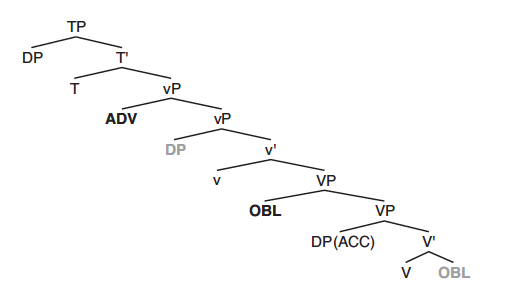
\includegraphics[width=4.1492in,height=2.2945in,width=\textwidth]{antonyyuk-img001.png}
 
\end{styleStandard}

\begin{styleStandard}
\textit{\newline
Figure 1: Derived order of a Group 1 verb.}
\end{styleStandard}

\begin{styleStandard}
Testing this prediction with a Group 1 predicate we get the following results:
\end{styleStandard}

\begin{styleinnerExample}
(48)\textbf{ \ \ }a.\ \ \textit{Maša \ \ special’no \ \ \ potrebovala s \ \ \ \ \ \ Ivana \ \ \ \ \ dengi~}
\end{styleinnerExample}

\begin{styleinnerExample}
\ \ \ \ Masha purposefully demanded \ \  \ from Ivan\textsc{ gen~}money\textsc{ acc}
\end{styleinnerExample}

\begin{styleinnerExample}
\ \ \ \ “Masha demanded money~from Ivan”\newline

\end{styleinnerExample}

\begin{styleinnerExample}
\ \ b.\ \ \textit{*Maša \ \ potrebovala \ s \ \ \ \ \ \ Ivana \ \ \ \ \ \ special’no dengi}~
\end{styleinnerExample}

\begin{styleinnerExample}
\ \ \ \  \ Masha purposefully from Ivan\textsc{{}-gen~}demanded \ money\textsc{ acc}
\end{styleinnerExample}

\begin{styleStandard}
Note that the structure in Figure 1 is identical to that proposed for Russian ditransitives in Bailyn (1995), (2012) based on independent types of evidence, thus our conclusions here converge with previous research.\footnote{ The conclusions regarding the base-generated order of Group 1 (and Group 3) verbs also converge with the findings reported in Titov (2017), who argues that once Information-Structural considerations licensing various derived word orders in Russian are controlled for, the “canonical” order of Russian ditransitive verbs emerges, that being the ACC {\textgreater} DAT order (see also Cepeda \& Cyrino, this volume, for a similar conclusion regarding Spanish, European Portuguese and Brazilian Portuguese). Note, however, that the general results reported here contradict the conclusions of Titov (2017), as it is shown here that there is no homogeneity among Russian ditransitives, with Group 2 verbs having a different base-generated order which is reflected in significant differences in their syntactic behavior, something Titov’s account has nothing to say about. Thus, one of the verbs Titov discusses, \textit{podvergnut’}, is a typical Group 2 verb, whereas Titov argues for the same ACC {\textgreater}{\textgreater} DAT base order for this and all other verbs she considers and furthermore argues that these conclusions hold quite generally for all ditransitive predicates in Russian. To the extent that the conclusions reached in this paper are correct, however, they suggest that while controlling for Information Structure licensing may be necessary, it will not be sufficient to correctly determine verbal argument structure and that QP scope distribution patterns provide a more accurate diagnostic of internal argument structure. }
\end{styleStandard}

\begin{listWWNumxxivleveli}
\item 
\begin{listWWNumxxivlevelii}
\item 
\begin{stylelsSectionii}
Possible structures for group 2 predicates
\end{stylelsSectionii}
\end{listWWNumxxivlevelii}
\end{listWWNumxxivleveli}
\begin{styleStandard}
We have seen that assuming the correctness of SFG entails that the Accusative-marked object of Group 2 verbs must be generated lower than the Oblique-marked argument (see 49 below). I have proposed in Antonyuk (2015) that this is due to the fact that the low Accusative is not a true direct object, but is effectively an Oblique argument base-generated low inside a PP, with a silent P head assigning it lexical Accusative case. 
\end{styleStandard}

\begin{styleStandard}
(49)
\end{styleStandard}

\begin{styleStandard}
V ~ NP (ACC) NP-OBL~~~NP (ACC)\ \ DERIVED ORDER (frozen) \ ~ \ \ \ \ \ \ \ \ \ \ \ \ \ \ \ \ \ \ \ \ \ \ \ \ \ \ \ \ \ \ {\textbackslash}\_\_\_\_\_\_\_\_\_\_\_\_\_\_\_\_\_\_\_\_\_/
\end{styleStandard}

\begin{styleStandard}
Regarding the structural possibilities themselves, as was already noted, they appear to be quite similar to those available for Group 1 verbs:
\end{styleStandard}

\begin{styleinnerExample}
(50)\textbf{\ \ }a. \ \ [PP P DP\textsc{acc~}] raises over OBL and adjoin to VP
\end{styleinnerExample}

\begin{styleinnerExample}
\ \ b. \ \ [PP P DP\textsc{acc~]}\textsubscript{ }raises over OBL to Spec,ApplP.
\end{styleinnerExample}

\begin{styleStandard}
In terms of the Agent-oriented adverbs, the two Groups behave alike, which means analyses requiring high adjunction with concomitant v-to-T raising are highly unlikely:
\end{styleStandard}

\begin{styleinnerExample}
(51)\textbf{ \ \ }a.\ \ \textit{Maša \ \ special’no \ \ \ obozvala [vrednogo \ malčika] (nexorošim}
\end{styleinnerExample}

\begin{styleinnerExample}
\ \ \ \ Masha purposefully called \ \ \ \ \ [capricious boy]\textsc{acc }[bad
\end{styleinnerExample}

\begin{styleinnerExample}
\textsc{\ \ \ \ }\textit{slovom)}
\end{styleinnerExample}

\begin{styleinnerExample}
\ \ \ \ word]\textsc{instr}
\end{styleinnerExample}

\begin{styleinnerExample}
\ \ \ \ “Masha purposefully called a capricious boy with a bad word”
\end{styleinnerExample}

\begin{styleinnerExample}
\ \ b.\ \ \textit{*Maša \ obozvala [vrednogo malčika] \ special’no \ \ \ \ \ (nexorošim }
\end{styleinnerExample}

\begin{styleinnerExample}
\ \ \ \  \ Masha called \ \ \ \ [capricious boy]\textsc{acc~} purposefully \ [bad
\end{styleinnerExample}

\begin{styleinnerExample}
\textsc{\ \ \ \ }\textit{slovom)}
\end{styleinnerExample}

\begin{styleinnerExample}
\ \ \ \ word]\textsc{instr}
\end{styleinnerExample}

\begin{styleinnerExample}
\ \ \ \ “Masha purposefully called a capricious boy with a bad word”
\end{styleinnerExample}

\begin{styleStandard}
Given these considerations, the structure of a sentence such as (52a) would seem to be something like in Figure 2, where the sentence contains two oblique complements (a DP and a PP).
\end{styleStandard}

\begin{styleinnerExample}
(52)\textbf{ \ \ }a.\ \ \textit{Maša \ \ ugostila (kakim-to pečenjem) \ \ \ \ \ každogo rebenka}
\end{styleinnerExample}

\begin{styleinnerExample}
\ \ \ \ Masha treated \ \ [some \ \ \ \ \ \ cookie]\textsc{instr}[every \ \ \ \ child]\textsc{acc}
\end{styleinnerExample}

\begin{styleinnerExample}
\ \ \ \ “Masha treated every child to some cookie” ${\exists}{\forall}$/${\forall}{\exists}$
\end{styleinnerExample}

\begin{styleinnerExample}
\ \ b.\ \ \textit{Maša \ \ ugostila [kakogo-to rebenka] \ (každym pečenjem)}
\end{styleinnerExample}

\begin{styleinnerExample}
\ \ \ \ Masha treated \ \ [some \ \ \ \ \ \ \ \ child]\textsc{acc~}[every \ \ \ cookie]\textsc{instr}
\end{styleinnerExample}

\begin{styleinnerExample}
\ \ \ \ “Masha treated some child to every cookie” ${\exists}{\forall}$/*${\forall}{\exists}$
\end{styleinnerExample}

\begin{styleStandard}
\textbf{Figure 2. }
\end{styleStandard}

\begin{styleStandard}
  [Warning: Image ignored] % Unhandled or unsupported graphics:
%\includegraphics[width=4.6165in,height=1.7866in,width=\textwidth]{antonyyuk-img002.emf}
 
\end{styleStandard}

\begin{styleStandard}
\textit{Figure 2: Base order of a Group 2 verb.}
\end{styleStandard}

\begin{styleStandard}
The frozen order would then be derived by fronting the PP, presumably by left-adjoining it to VP as in Figure 3.\footnote{ In Figure 3 the lower PP copy is of course taken to be silent. } 
\end{styleStandard}

\begin{styleStandard}
\textbf{Figure 3.}
\end{styleStandard}

\begin{styleStandard}
  [Warning: Image ignored] % Unhandled or unsupported graphics:
%\includegraphics[width=4.6165in,height=1.2972in,width=\textwidth]{antonyyuk-img003.emf}
 
\end{styleStandard}

\begin{styleStandard}
\textit{Figure 3: Derived order of a Group 2 verb.}
\end{styleStandard}

\begin{styleStandard}
Incidentally, there is further evidence for the proposal that Group 2 predicates involve two oblique phrases. Consider (53):
\end{styleStandard}

\begin{styleinnerExample}
(53)\textbf{ \ \ }a.\ \ \textit{Maša \ pobesedovala na kakuju-to temu) \ \ \ \ \ \ \ \ \ \ \ \ [s \ \ \ \ \ \ každym}
\end{styleinnerExample}

\begin{styleinnerExample}
\ \ \ \ Masha talked. \ \ \ \ [\textsubscript{PP} \ on [some \ \ \ \ \ topic]\textsc{acc }][\textsubscript{PP} with [every 
\end{styleinnerExample}

\begin{styleinnerExample}
\textit{\ \ \ \ drugom]}
\end{styleinnerExample}

\begin{styleinnerExample}
\ \ \ \ friend]\textsc{instr}]
\end{styleinnerExample}

\begin{styleinnerExample}
\ \ \ \ “Masha had a conversation on some topic with every friend” ${\exists}{\forall}$/${\forall}{\exists}$
\end{styleinnerExample}

\begin{styleinnerExample}
\ \ b.\ \ \textit{Maša. \ pobesedovala [s \ \ \ \ \ \ kakim-to drugom] \ \ \ \ \ \ \ \ \ \ \ (na každuju-to }
\end{styleinnerExample}

\begin{styleinnerExample}
\ \ \ \ Masha talked \ \ \ \ \ \ \ \ [\textsubscript{PP} with [some \ \ \ \ \ friend]\textsc{instr}] [\textsubscript{PP} on [every 
\end{styleinnerExample}

\begin{styleinnerExample}
\textit{\ \ \ \ temu)}
\end{styleinnerExample}

\begin{styleinnerExample}
\ \ \ \ topic]\textsc{acc}]
\end{styleinnerExample}

\begin{styleinnerExample}
\ \ \ \ “Masha had a conversation with some friend on every topic ${\exists}{\forall}$/*${\forall}{\exists}$
\end{styleinnerExample}

\begin{styleStandard}
The example in (53) contains a ditransitive predicate with two overt quantificational PPs, with one of those Ps assigning Accusative case. Thus, this example is fully analogous to what I suggest for Group 2 predicates, the only difference being that the preposition assigning Accusative is overt in (53) but covert in all the other cases we’ve seen in this section. Finally, the strongest piece of evidence in support of the proposal that there is in fact a null P assigning Accusative case in a low position in Group 2 predicates is examples such as (54):
\end{styleStandard}

\clearpage\begin{styleinnerExample}
(54)\textbf{\ \ }a.\ \ \textit{Maša \ \ otrugala \ \ \ (za \ kakuju-to ošibku) \ \ \ \ \ \ \ \ \ [každogo druga]}
\end{styleinnerExample}

\begin{styleinnerExample}
\ \ \ \ Masha scolded [\textsubscript{PP }for [some \ \ \ \ \ \ mistake]\textsc{acc}] [every \ \ \ friend]\textsc{acc~}
\end{styleinnerExample}

\begin{styleinnerExample}
\ \ \ \ “Masha scolded every friend for some mistake” ${\exists}{\forall}$/${\forall}{\exists}$\newline

\end{styleinnerExample}

\begin{styleinnerExample}
\ \ b.\ \ \textit{Maša \ \ otrugala [kakogo-to druga] \ \ \ \ \ \ \ \ \ \ \ (za \ každuju \ ošibku)}
\end{styleinnerExample}

\begin{styleinnerExample}
\ \ \ \ Masha scolded \ [some \ \ \ \ \ \ \ \ friend]\textsc{acc} [\textsubscript{PP} for [every \ \ \ \ mistake]\textsc{acc}]
\end{styleinnerExample}

\begin{styleinnerExample}
\ \ \ \ “Masha scolded some friend for every mistake” ${\exists}{\forall}$/*${\forall}{\exists}$
\end{styleinnerExample}

\begin{styleStandard}
What is interesting about this example, and of utmost importance for the structural analysis advanced here, is the following: this ditransitive verb “otrugat’’ (‘to scold’) selects two Accusative-marked objects, one Oblique, occurring inside an overt Prepositional Phrase and one which looks like a regular direct object Accusative. However, the scope pattern that we find with this pair of examples, specifically the frozen scope status of (54b), suggests that (54b) is the \textit{derived }order, that is, what looks like the regular direct object Accusative must have originated below the Accusative that is inside the PP. This, of course, on my assumptions suggests that the “regular” direct object Accusative in (54b) is in fact a concealed low Oblique Accusative, which originates inside a null PP and thus gets its case from a null P head. Significantly, the above “direct object” Accusative argument does not do well on the objecthood tests discussed before:
\end{styleStandard}

\begin{styleinnerExample}
(55)\textbf{\ \ }a.\ \ \textit{*Maša \ otrugala po drugu za každuju \ \ \ \ \ \ \ \ \ \ \ \ ošibku }
\end{styleinnerExample}

\begin{styleinnerExample}
\textbf{\ \  \ }Masha scolded \ po friend-\textsc{dat} [\textsubscript{PP} for [every mistake]\textsc{acc~}]
\end{styleinnerExample}

\begin{styleinnerExample}
\textbf{\ \ \ \ \ \ \ \ \ \ \ \ \ \  \ Distributive po test}\newline
b.\ \ \textit{??Maša \ \ \ ne. \ \ \ otrugala podrugi} \ \ \ \ \ \textbf{Genitive of Negation}
\end{styleinnerExample}

\begin{styleinnerExample}
\ \ \ \  \ \ \ Masha NEG scolded \ \ girlfriend-\textsc{gen\newline
}
\end{styleinnerExample}

\begin{styleinnerExample}
\ \ c.\ \ \textit{*Maša \ \ \ dorugalas’. \ \ \ \ \ \ \ \ druga do togo, čto \ on ušel} \ \ \ \ \ \ \ \ \ \ \ \ \ \ \ \ \ \ \ \textbf{RUR}
\end{styleinnerExample}

\begin{styleinnerExample}
\ \ \ \  \ Masha \ DO-scold-REFL friend to \ that \ that \ he left
\end{styleinnerExample}

\begin{styleinnerExample}
\ \ \ \ “Masha scolded her friend into leaving”
\end{styleinnerExample}

\begin{styleinnerExample}
\ \ d.\ \ \textit{Maša \ \ \ dorugalas’} \ \ \ \ \ \ \ \ \ \  \ \ \ \ \ \ \ \ \ \ \ \textbf{RIR} (Tatevosov 2010)
\end{styleinnerExample}

\begin{styleinnerExample}
\ \ \ \ Masha \ DO-scold-REFL
\end{styleinnerExample}

\begin{styleinnerExample}
\ \ \ \ “Masha scolded her way to some negative result”
\end{styleinnerExample}

\begin{styleStandard}
As the above tests show, the Accusative-marked object does not behave as would be expected of a true direct object: it does not allow the distributive \textit{po} phrase, is strongly degraded in the Genitive of Negation configuration and the Unaccusative Resultative built on it is ungrammatical while the Intensive Resultative is, as expected. The conclusion is therefore that this particular predicate does not subcategorize for a direct object but instead takes two Oblique arguments, one of which is an overt PP, with the preposition \textit{za} marking its complement with lexical Accusative case, and another oblique argument which is also assigned lexical Accusative case, by a silent P head.\footnote{ In Antonyuk (in prep.) I show that while not all psychological verbs (Belletti \& Rizzi 1988) allow alternating (causative) ditransitive forms, those that do necessarily form Group 2 ditransitives. Note further that while the homogeneous behavior of Group 2 verbs with respect to the unaccusativity diagnostics suggests a certain homogeneity within the Group in terms of syntactic structure, it is certainly not the case that all Group 2 verbs are psych verbs. Thus to the extent that theories arguing that the Causer argument is generated in Spec, vP while the Agent is generated in Spec, VoiceP, (see Kratzer 2005 and Alexiadou et al. 2006 i.a.), the verbs belonging to Group 2 are expected to differ with respect to the position of the higher internal argument (e.g., Spec, VP for non-Causers/Themes vs Spec,vP for Causers).}
\end{styleStandard}

\begin{listWWNumxxivleveli}
\item 
\begin{listWWNumxxivlevelii}
\item 
\begin{stylelsSectionii}
Structural possibilities for group 3 predicates
\end{stylelsSectionii}
\end{listWWNumxxivlevelii}
\end{listWWNumxxivleveli}
\begin{styleStandard}
With regard to Group 3 predicates, there are two major possibilities: independent projection or a derivational relation between the two alternating orders of internal arguments. While the scope ambiguity of both orders, coupled with SFG might suggest that the two orders are independently projected, I argue this is not the case. Consider (56):
\end{styleStandard}

\begin{styleinnerExample}
(56)\textbf{ \ \ }a.\ \ Job blamed [God] [for his troubles] \ \ (Larson 1990)
\end{styleinnerExample}

\begin{styleinnerExample}
\ \ b.\ \ Job blamed [his troubles] [on God]
\end{styleinnerExample}

\begin{styleStandard}
What makes these good candidates for independent projection is the fact that along with the change in the order of the two internal arguments, there is also clearly a change in grammatical relations, with ‘God’ being a DO in (56a) but an oblique in (56b). As noted by Richard Larson (p.c.), the corresponding examples with quantificational phrases are both ambiguous, as expected under my analysis:
\end{styleStandard}

\begin{styleinnerExample}
(57)\textbf{ \ \ }a.\ \ John blamed some employee for every mistake. \ \ ${\exists}{\forall}$,${\forall}{\exists}$\ \ \newline
b. \ \ John blamed some mistake on every employee. \ \ ${\exists}{\forall}$,${\forall}{\exists}$\newline

\end{styleinnerExample}

\begin{styleStandard}
Native speakers apparently also perceive an additional semantic distinction between these, as well, with (57a) being notationally related to (58a), and (57b) being related to locatives, as in (58b):
\end{styleStandard}

\begin{styleinnerExample}
(58)\textbf{\ \ }a.\ \ John thanked some employee for every success.\newline
b.\ \ John gave/offered thanks to some employee for every success.
\end{styleinnerExample}

\begin{styleStandard}
The fact that the thematic roles involved in the two alternations are different in the above cases supports the idea that they are not derivationally related. This poses a problem for the non-derivational account of Group 3 ditransitive alternations since in none of them can a parallel difference in thematic roles be detected. The only differences seem to be related to the information structural status of the two internal arguments, with their thematic roles always staying the same. Thus, it is worth considering other alternatives. With independent projection arguably ruled out and the movement of the kind implicated with Groups 1 and 2 being excluded by the fact that both orders are scopally ambiguous, I suggest that orders such as (59b) are derived via Light Predicate Raising (LPR) (following Larson 1989; 2014).
\end{styleStandard}

\begin{styleinnerExample}
(59)\textbf{\ \ }a.\ \ \textit{Maša \ napisala [kakoj-to slogan] \ \ \ \ \ \ \ \ (na každoj stene)} ${\exists}{\forall}$/${\forall}{\exists}$
\end{styleinnerExample}

\begin{styleinnerExample}
\ \ \ \ Masha wrote. \ \ \ [some \ \ \ \ slogan]\textsubscript{ACC} [\textsubscript{PP} on [every wall]\textsc{prep }]
\end{styleinnerExample}

\begin{styleinnerExample}
\ \ \ \ “Masha wrote some slogan on every wall”
\end{styleinnerExample}

\begin{styleinnerExample}
\ \ b.\ \ \textit{Maša napisala \ (na \ kakoj-to stene) \ \ \ \ \ \ \ [každyj slogan]} \ ${\exists}{\forall}$/${\forall}{\exists}$
\end{styleinnerExample}

\begin{styleinnerExample}
\ \ \ \ Masha wrote [\textsubscript{PP} on [some \ \ \ \ wall]\textsc{prep}] [every slogan]\textsubscript{ACC}
\end{styleinnerExample}

\begin{styleinnerExample}
\ \ \ \ “Masha wrote every slogan on some wall”
\end{styleinnerExample}

\begin{styleStandard}
Consider the derivation of (59b) in Figure 4 below:
\end{styleStandard}

\begin{styleStandard}
\textbf{Figure 4.}
\end{styleStandard}

\begin{styleStandard}
  [Warning: Image ignored] % Unhandled or unsupported graphics:
%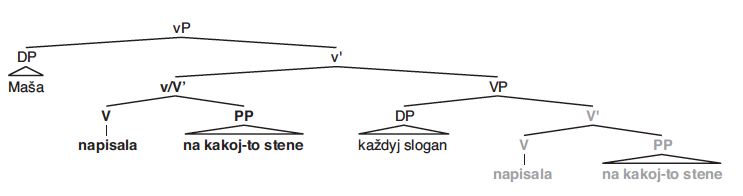
\includegraphics[width=4.7492in,height=1.2528in,width=\textwidth]{antonyyuk-img004.png}
 
\end{styleStandard}

\begin{styleStandard}
\textit{Figure 4: Derived order of a Group 3 verb.}
\end{styleStandard}

\begin{styleStandard}
As evident from structural relations in Figure 4, what is crucially important in relation to my analysis is that the LPR configuration does not lead to a situation where the raised PP/DP is able to c-command the other phrase, by virtue of the interfering v/V' node, thus accounting for the lack of scope freezing in these examples.
\end{styleStandard}

\begin{styleStandard}
\ \ While adopting Larson's LPR analysis provides a straightforward way to account for the lack of scope freezing with Group 3 verbs, in the absence of an independent motivation for the application of such LP Raising with verbs belonging to this group, its adoption here to account for the apparent violation of the SFG with these verbs might seem too stipulative to be persuasive. However, I will argue here that Group 3 predicates are different from those in Group 2 and even from the very similar Group 1 verbs in important respects which explains their syntactic behavior. A careful examination of Group 3 verbs listed in (18) reveals that all such predicates (to the exclusion of a few verbs to be discussed shortly) share the property of taking a direct object marked with structural Accusative case and a Preposition Phrase. I argue that it is precisely the nature of the PP complement that plays the crucial role here and provides an explanation for the observed differences between Group 1 and Group 3. The limited class of PPs observed with Group 3 predicates can be characterized as sharing the property of signifying either direction (of movement) or location (\textit{v/in, na/on, ot/from, iz/from/ k/to }or\textit{ towards}). Thus, Group 3 is crucially similar to Group 1 verbs in subcategorizing for a direct object DP marked with structural Accusative case, but unlike Group 1 verbs, Group 3 verbs take a locational/directional PP complement (whereas Group 1 verbs take a Dative case-maked DP complement or a PP which takes a relational preposition (\textit{s/from, s/with, dlja/for}). To put this into terminology used in research on prepositional phrases, Group 3 PPs are those where the P introduces the Ground argument (see Svenonius 2003, 2007 and related research). Group 1 prepositional heads, being strictly relational, do not. Finally, another similarity between Groups 1 and 3 which at first glance might suggest that the above differentiation is unjustified, is due to the fact that some verbs classified as Group 3 are verbs like \textit{otdat' }(to give away, to give back), which take an ACC-marked THEME and a DAT-marked GOAL argument, just like the numerous ACC/DAT verbs that belong to Group 1. \textit{Otdat'}, in fact, is related to the verb \textit{dat' }(give), which is a canonical Group 1 ditransitive that exhibits scope freezing on the DAT{\textgreater}ACC order of internal arguments (also discussed in Boneh and Nash 2017). As discussed in Antonyuk (2015), such Group 3 verbs present particular difficulties during classification attempts due to showing strong surface scope bias on DAT{\textgreater}ACC order, which often leads to their initial misclassification as Group 1 verbs. However, additional tests, such as the use of Constrastive Focus (Antonyuk and Larson 2016) help establish that they are in fact Group 3 verbs. Here I argue that the (lexical) prefixes verbs such as \textit{otdat'} occur with is the very reason they behave as Group 3 verbs, unlike their unprefixed Group 1 counterparts. The prefixes taken by Group 3 verbs are crucially distinct from whatever prefixes (if any) may be found with Group 1 or Group 2 verbs in signifying direction/location, just like the PPs that occur as complements of Group 3 verbs do. The unified semantics of the class of the prepositions and prefixes that appear with Group 3 verbs suggests a natural way of explaining their behavior. If prepositions and prefixes are both elements of category P (Matushansky 2002; Biskup 2017; and esp. Svenonius 2004, 2008), then one might argue that the empirical observation that locational/directional prepositions behave in some sense as being \textit{closer} to the verb than other prepositions (including preposition \textit{to} in English which occurs in PP Dative constructions)\footnote{ As pointed out to me by Larson (p.c.).} may be explained by the need of such prepositions (and the PPs they project) to occur at LF as syntactic units with the verb. There are two ways in which this can be achieved: either the PP raises and attaches to the verb at LF (which is arguably what happens with Group 3 verbs on their basic order), or the verb raises to its position inside the vP together with the PP, which is exactly what happens in cases of Light Predicate Raising. If the latter option is employed, scope freezing does not take place and the lower QP is then free to raise above the structurally higher one at LF, which then accounts for the ambiguous nature of the derived word order with Group 3 predicates, but not with Group 1 and 2. Thus, while the account sketched here needs to be fleshed out, it suggests an intuitive explanation for why Group 3 verbs pattern differently from Groups 1 and 2 as far as QP scope is concerned.
\end{styleStandard}

\begin{listWWNumxxivleveli}
\item 
\begin{stylelsSectioni}
Conclusions
\end{stylelsSectioni}
\end{listWWNumxxivleveli}
\begin{styleStandard}
I have argued that the argument structure of ditransitives can be studied by considering their quantifier scope ambiguity and scope freezing distribution patterns. Assuming the Scope Freezing Generalization is correct and using it to probe argument structure affords us novel insights and suggests that Russian ditransitives are not a homogeneous group, but in fact subdivide into three distinct Groups, each associated with a distinct structure and a distinct set of properties. Most importantly, however, the data discussed here provide strong evidence that not all “direct objects” are in fact true direct objects with expected properties: the data presented here suggest that a whole group of such objects are in fact concealed Obliques. The derivational account of Russian ditransitives offered in this paper has a number of important consequences, with implications for argument structure, verbal alternations, the status of directional/location PPs as a natural class, the notion of ditransitivity and the status of Light Predicate Raising in the grammar that are left largely without discussion due to space limitations.\footnote{ Note that Cepeda \& Cyrino (this volume) and Cornilescu (this volume) similarly offer derivational accounts of ditransitives in Spanish, European Portuguese, Brazilian Portuguese and Romanian respectively. To the extent that these papers focus on the more prototypical ditransitives that on my account belong to Group 1 predicates where I argue ACC {\textgreater} DAT or DO {\textgreater} IO order is base-generated, our conclusions seem to converge. Cepeda and Cyrino (this volume) additionally argue that Spanish, European Portuguese and Brazilian Portuguese do not have a DOC, primarily based on the fact that IOs do not passivize in these languages. While passivization is not discussed in my paper, IOs in Russian (and East Slavic more generally) do passivize, thus pointing to a genuine difference in this respect between the languages under consideration.} 
\end{styleStandard}

\begin{listWWNumxxivleveli}
\item 
\begin{stylelsSectioni}
References
\end{stylelsSectioni}
\end{listWWNumxxivleveli}
\begin{styleStandard}
Alexiadou Artemis, Anagnostopoulou Elena \& Schäfer Florian. 2006. The properties of anticausatives crosslinguistically. In Phases of Interpretation, Mara Frascarelli (ed.), 187–211. Berlin: Mouton de Gruyter.
\end{styleStandard}

\begin{styleStandard}
Antonyuk, Svitlana. in preparation. Psych Verb Alternations in (East) Slavic. Ms. University of Vienna.
\end{styleStandard}

\begin{styleStandard}
Antonyuk, Svitlana. 2019. Quantifier Scope in Russian. \textit{Glossa: A Journal of General Linguistics, 4}(1), 54. DOI://http.doi.org/10.5334/gjgl.562
\end{styleStandard}

\begin{styleStandard}
Antonyuk, Svitlana \& Roksolana Mykhaylyk. under review. Scope Freezing and Object Shift in Ukrainian: does Superiority Matter? Remark.
\end{styleStandard}

\begin{styleStandard}
Antonyuk, Svitlana. 2018. Embracing the Differences: the Three Classes of Russian Ditransitives. \textit{Proceedings of Formal Approaches to Slavic Linguistics} (FASL) 25, Cornell University, Ithaca, New York.
\end{styleStandard}

\begin{styleStandard}
Antonyuk, Svitlana. 2017. How QP Scope Can Weigh in on a Long-Time Debate: the Puzzle of Russian Ditransitives. In \textit{A Pesky Set: Papers for David Pesetsky}. Eds. Claire Halpert, Hadas Kotek, Coppe van Urk. Massachusetts Institute of Technology Working Papers in Linguistics (MITWPL) special volume, CreateSpace Independent Publishing Platform, 566p.
\end{styleStandard}

\begin{styleStandard}
Antonyuk, Svitlana \& Richard Larson. 2016. Scope Freezing in PP Dative Constructions? Presentation given at Formal Description of Slavic Languages 12 (FDSL), Humboldt University, Berlin, German
\end{styleStandard}

\begin{styleStandard}
Antonyuk, Svitlana. 2015. \textit{Quantifier Scope and Scope Freezing in Russian}. Doctoral dissertation, Stony Brook University, Stony Brook, NY.
\end{styleStandard}

\begin{styleStandard}
Antonyuk-Yudina, Svitlana. 2006. The Scope of Quantifier Phrases in Russian: A QR Analysis. Linguistics in the Big Apple: online proceedings of SUNY/CUNY/NYU/Yale.
\end{styleStandard}

\begin{styleStandard}
Bailyn, John. 2012. \textit{The Syntax of Russian.} Cambridge University Press.
\end{styleStandard}

\begin{styleNormalWeb}
Bailyn, John. 2010. What’s Inside VP? New (and Old) Evidence from Russian. In Wayles Browne et al. (eds.), \textit{Formal Approaches to Slavic Linguistics }18: The Second Cornell Meeting, Ann Arbor, MI: Michigan Slavic Publications. 
\end{styleNormalWeb}

\begin{styleStandard}
Bailyn, John. 1995. \textit{A Configurational Approach to Russian “Free” Word Order}. Doctoral dissertation, Cornell University, Ithaca, NY.
\end{styleStandard}

\begin{styleNormalWeb}
Belletti, Andriana \& Luigi Rizzi. 1988. Psych-verbs and theta theory. \textit{Natural Language and Linguistic Theory} 6: 291-352. 
\end{styleNormalWeb}

\begin{styleNormalWeb}
Biskup, Petr. 2017. \textit{Prepositions and Verbal Prefixes: The Case of Slavic}. Habilitation. Universität Leipzig.
\end{styleNormalWeb}

\begin{styleNormalWeb}
Boneh, Nora \& Léa Nash. 2017. The syntax and semantics of dative DPs in Russian ditransitives. Natural Language and Linguistic Theory 35:4, 899-953.
\end{styleNormalWeb}

\begin{styleStandard}
Bruening, Benjamin. 2010. Double Object Constructions Disguised as Prepositional Datives.~~\textit{Linguistic Inquiry}~41: 287-305.
\end{styleStandard}

\begin{styleStandard}
Bruening, Benjamin. 2001. QR Obeys Superiority: ACD and Frozen Scope. \textit{Linguistic Inquiry} \ 32(2):233-273.
\end{styleStandard}

\begin{styleStandard}
Dyakonova, Marina. 2007/2009. \textit{A Phase-based Approach to Russian Free Word Order}. Doctoral dissertation. University of Amsterdam. 
\end{styleStandard}

\begin{styleStandard}
Dyakonova, Marina. 2005. Russian Double Object Constructions. \textit{Amsterdam Center for Language and Communication Working Papers }2(1): 3–30. 
\end{styleStandard}

\begin{styleStandard}
Franks, Steven. 1995. \textit{Parameters of Slavic Morphosyntax}. New York / Oxford: Oxford University Press.
\end{styleStandard}

\begin{styleStandard}
Greenberg, Gerald \& Steven Franks. 1991. A Parametric Approach to Dative Subjects and the Second Dative in Slavic. The Slavic and East European Journal 35:1, 71-97.
\end{styleStandard}

\begin{styleStandard}
Hallman, Peter. 2015. Syntactic Neutralization in Double Object Constructions. \textit{Linguistic Inquiry} 46: 389-424.
\end{styleStandard}

\begin{styleStandard}
Harbert, Wayne \& Almeida Toribio. 1991. Nominative Objects. \textit{Cornell Working Papers in Linguistics }9: 127–192. 
\end{styleStandard}

\begin{styleStandard}
Harley, Heidi. 2002. Possession and the double object construction. \textit{Linguistic Variation Yearbook} 2, 31-70
\end{styleStandard}

\begin{styleStandard}
Harley, Heidi. 1995. \textit{Subjects, Events and Licensing}. Doctoral dissertation, MIT, Cambridge, MA. 
\end{styleStandard}

\begin{styleStandard}
Irvin, Patricia. 2012 Unaccusativity at the Interfaces. Doctoral dissertation, New York University.
\end{styleStandard}

\begin{styleStandard}
Kratzer, Anjelika. 2005. Building resultatives. In \textit{Event Arguments: Foundations and Applications}, ed. Claudia Maienborn and Angelika Wöllstein-Leisten, 177– 212. T\"{u}bingen: Max Niemeyer Verlag.
\end{styleStandard}

\begin{styleStandard}
Larson, Richard 2014. \textit{On Shell Structure}. Routledge, London.
\end{styleStandard}

\begin{styleStandard}
Larson, Richard. 1990. Double Objects Revisited: Reply to Jackendoff. \textit{Linguistic Inquiry} 21: 589-632.
\end{styleStandard}

\begin{styleStandard}
Larson, Richard. 1989. Light Predicate Raising. 1989. \textit{MIT Lexicon Project Working Papers} 27. 
\end{styleStandard}

\begin{styleStandard}
Larson, Richard. 1988. On the Double Object Construction. \textit{Linguistic Inquiry} 19: 335–391. 
\end{styleStandard}

\begin{styleStandard}
Levin, Beth \& Malka Rappaport Hovav. 1995. \textit{Unaccusativity.} Cambridge MA: MIT Press.
\end{styleStandard}

\begin{styleStandard}
Marantz, Alec. 1993. Implications of Asymmetries in Double Object Construction. In Sam Mchombo (ed.), Theoretical Aspect of Bantu Grammar, CSLI Publications, Stanford, California, pp. 113-150. 
\end{styleStandard}

\begin{styleStandard}
Matushansky, Ora. 2002. On Formal Identity of Russian Prefixes and Prepositions. \textit{MIT Working Papers in Linguistics} 42, 217-253
\end{styleStandard}

\begin{styleStandard}
Pesetsky, David. 1995. Zero Syntax. Cambridge, Mass.: MIT Press.
\end{styleStandard}

\begin{styleStandard}
Pesetsky, David. 1982. Paths and Categories. Doctoral dissertation, MIT, Cambridge, MA.
\end{styleStandard}

\begin{styleStandard}
Pylkk\"{a}nen, Liina. 2002. \textit{Introducing Arguments}. Doctoral dissertation, MIT, Cambridge, MA. 
\end{styleStandard}

\begin{styleStandard}
Rappaport Hovav, Malka \& Beth Levin. 2001. An Event Structure Account of English Resultatives.~\textit{Language}~77, 766-797.
\end{styleStandard}

\begin{styleStandard}
Richardson, Kylie. 2007. \textit{Case and Aspect in Slavic. }Oxford: Oxford University Press. 
\end{styleStandard}

\begin{styleStandard}
Svenonius, Peter. 2008. Russian Prefixes are Phrasal. In \textit{Formal~Description of Slavic Languages, }edited by Gerhild Zybatow, Luka Szucsich, Uwe Junghanns, and Roland Meyer, pp. 526-537. Peter Lang, Frankfurt am Main. 
\end{styleStandard}

\begin{styleStandard}
Svenonius, Peter. 2007. Adpositions, Particles, and the Arguments~they Introduce. In \textit{Argument~Structure, }ed. By Eric Reuland, Tanmoy Bhattacharya, and Giorgos Spathas, pp. 63-103. John Benjamins, Amsterdam.
\end{styleStandard}

\begin{styleStandard}
Svenonius, Peter. 2004. Slavic Prefixes and Morphology. \textit{Nordlyd~}32.2: 177-204.
\end{styleStandard}

\begin{styleStandard}
Tatevosov, Sergei. 2010. Building Intensite Resultatives. In Browne W. (ed.) \textit{Formal Approaches to Slavic Linguistics} (FASL). The Cornell Meeting. Ann Arbor: Michigan Slavic Publications, 289- 302.
\end{styleStandard}

\begin{styleStandard}
Titov, Elena. 2017. The Canonical Order of Russian Objects. \textit{Linguistic Inquiry} 48:3, 427-457
\end{styleStandard}

\end{document}
